%%
%% ACM Computing Surveys (CSUR) — main manuscript
%% Template: acmart.cls
%% Formatting reference: Cao (2025) ACM Computing Surveys, DOI:10.1145/3770574
%%
%% NOTE: Use \documentclass[manuscript,screen]{acmart} for submission draft;
%%       switch to \documentclass[acmjour]{acmart} for camera-ready.

\documentclass[manuscript,screen]{acmart}

%% Remove copyright box for draft
\setcopyright{none}
\acmDOI{}
\acmISBN{}
\acmJournal{CSUR}
\acmYear{2026}
\acmVolume{0}
\acmNumber{0}
\acmArticle{0}
\acmMonth{0}

%%----------------------------------------------------------------------
%% Packages
%%----------------------------------------------------------------------
\usepackage{booktabs}
\usepackage{multirow}
\usepackage{graphicx}
\usepackage{xcolor}
%% NOTE: hyperref is loaded internally by acmart — do NOT load it again
\usepackage{acronym}
\usepackage{afterpage}
% \usepackage{balance}  % enable for acmjour two-column camera-ready only

%%----------------------------------------------------------------------
%% Metadata
%%----------------------------------------------------------------------
\title{Humanoid Robots in Healthcare: Current Systems, Research Frontiers,
       and Clinical Opportunities}

\author{Anonymous Author(s)}
\affiliation{%
  \institution{[Institution Anonymized]}
  \city{[City Anonymized]}
  \country{[Country Anonymized]}
}
\email{[email anonymized]}

%%----------------------------------------------------------------------
%% Abstract
%%----------------------------------------------------------------------
\begin{abstract}
As of early 2026, modern commercial humanoid robots---bipedal, dexterous,
and large-language-model-capable---have demonstrated clinical task execution
in controlled laboratory settings, including teleoperated bimanual procedures
across seven clinical tasks~\cite{atar2025humanoids} and autonomous surgical
assistance in a cadaveric sphenoidectomy~\cite{cho2026humanoid}. Yet no
full-size bipedal humanoid robot holds FDA clearance or CE marking for any
clinical application, and no registered clinical trial has enrolled patients
for a study involving such a platform. This review is the first systematic
synthesis of the 2022--2026 humanoid-in-healthcare literature through a
clinical deployment lens. We surveyed five databases (arXiv, PubMed, IEEE
Xplore, ACM Digital Library, and Google Scholar), identifying 14 qualifying
peer-reviewed papers; assessed capabilities for 13 commercial and 12 academic
platforms; analyzed regulatory pathways under current FDA, EU MDR, and ISO
frameworks; and applied the ISO 16290:2013 Technology Readiness Level (TRL)
framework to five clinical application domains. All domains are at TRL 3--4;
the evidence base is concentrated on a single commercial platform (Unitree G1)
and a single research cluster (UC San Diego Yip Laboratory and Johns Hopkins
University). Three near-term roles have the strongest case for advancement to
TRL~5 within five years: telemedicine and telepresence clinical assistant,
rehabilitation movement demonstrator, and structured eldercare companion and
physical assistant. The primary barriers are not platform capability but the
absence of accepted safety standards for bipedal gait in patient-proximate
environments and the absence of registered human-subject feasibility
studies---the two gaps that must be resolved, in that order, before regulatory
engagement can begin.
\end{abstract}

\keywords{humanoid robots, healthcare robotics, embodied AI, large language
  models, human-robot interaction, clinical deployment, medical robots,
  technology readiness level, regulatory pathway}

\begin{CCSXML}
<ccs2012>
  <concept>
    <concept_id>10010520.10010553.10010562</concept_id>
    <concept_desc>Computer systems organization~Robotics</concept_desc>
    <concept_significance>500</concept_significance>
  </concept>
  <concept>
    <concept_id>10010147.10010178</concept_id>
    <concept_desc>Computing methodologies~Artificial intelligence</concept_desc>
    <concept_significance>300</concept_significance>
  </concept>
  <concept>
    <concept_id>10003456.10003462</concept_id>
    <concept_desc>Social and professional topics~Medical informatics</concept_desc>
    <concept_significance>300</concept_significance>
  </concept>
</ccs2012>
\end{CCSXML}

\ccsdesc[500]{Computer systems organization~Robotics}
\ccsdesc[300]{Computing methodologies~Artificial intelligence}
\ccsdesc[300]{Social and professional topics~Medical informatics}

\begin{document}

\maketitle

%%----------------------------------------------------------------------
%% Acronym definitions (must be inside document body, after \maketitle)
%%----------------------------------------------------------------------
\begin{acronym}
  \acro{AI}{Artificial Intelligence}
  \acro{LLM}{Large Language Model}
  \acro{VLM}{Vision-Language Model}
  \acro{VLA}{Vision-Language-Action Model}
  \acro{HRI}{Human-Robot Interaction}
  \acro{TRL}{Technology Readiness Level}
  \acro{ADL}{Activities of Daily Living}
  \acro{FDA}{U.S. Food and Drug Administration}
  \acro{ROS}{Robot Operating System}
  \acro{ICU}{Intensive Care Unit}
  \acro{AOT}{Action Observation Therapy}
  \acro{RCM}{Remote Center of Motion}
  \acro{PFL}{Power and Force Limiting}
  \acro{IRB}{Institutional Review Board}
  \acro{EHR}{Electronic Health Record}
  \acro{DOF}{Degrees of Freedom}
\end{acronym}

%%======================================================================
\section{Introduction}
\label{sec:intro}
%%======================================================================

The most capable humanoid robots ever built are commercially available today.
Figure~02, Boston Dynamics Atlas (electric), Tesla Optimus Gen~2, Unitree G1,
Fourier GR-2, and more than a dozen comparable platforms combine bipedal
locomotion, dexterous multi-fingered manipulation, and onboard sensing into
systems that operate in spaces designed for humans, handle objects designed for
human hands, and respond to instructions in natural language. Twelve of thirteen
major commercial humanoid platforms now integrate large language models directly
into their control architecture. In the laboratory, a Unitree G1 teleoperated by
a non-clinician completed seven distinct clinical procedures---auscultation,
ultrasound, IV catheter insertion, and four others---in a controlled experimental
setting~\cite{atar2025humanoids}; a second system operated as a surgical first
assistant in a cadaveric bilateral sphenoidectomy~\cite{cho2026humanoid}. Yet not
one of these systems holds FDA clearance or CE marking for any clinical
application. No registered Phase I, II, or III clinical trial has enrolled a
patient for a study involving a full-size bipedal humanoid platform. The
technical capability exists at a level that warrants serious clinical
investigation. The clinical deployment does not. This review examines why.

The disparity between demonstrated capability and clinical deployment is not a
permanent condition; it is a developmental phase. Two technological developments
converged after 2022 to move the humanoid healthcare question from speculative to
tractable. The first is hardware: commercial humanoid platforms crossed the
payload, dexterity, and locomotion threshold required to attempt clinical and
care tasks in their natural environments. Actuator and sensor configurations now
exist that allow manipulation of clinical instruments---stethoscopes, ultrasound
probes, laparoscopes---and navigation of clinical spaces at human working height
and stride. The second is software: the integration of large language models and
vision-language-action (VLA) models removed the per-task explicit programming
requirement that previously made general-purpose humanoid deployment impractical.
Instruction-following, task generalization, and adaptive response to unstructured
environments became achievable without the months-long engineering cycles that
earlier control architectures demanded. Both were necessary; neither alone was
sufficient. The result is a field that moved, in roughly three years, from
proof-of-concept locomotion demonstrations to laboratory execution of clinical
procedure sequences. The literature reviewed here covers that period: 2022 to
early 2026.

The existing review literature does not yet address this convergence. The closest
prior work is Cunha et al.~\cite{cunha2025humanoid}, a 2025 scoping review of 27
studies on care provided by humanoid robots, with a search cutoff of November
2023---predating the LLM/VLA integration that defines the current period
entirely. Earlier reviews of humanoid robots in healthcare~\cite{azeta2018review,mukherjee2022humanoid}
and service robots for healthcare delivery~\cite{ozturkcan2022humanoid,huang2023intelligent,morgan2022robots}
treat humanoid and non-humanoid platforms interchangeably, obscuring the
form-factor-specific barriers that determine clinical deployability. Embodied AI
reviews~\cite{liu2025screens,mir2026embodied,lisondra2026embodied} cover the
healthcare vertical as one application among many, without the
platform-specific and regulatory specificity that the clinical deployment
question requires. This review addresses the gap directly: it
is the first synthesis of the 2022--2026 humanoid-specific clinical and care
literature that integrates a platform capability assessment, a regulatory pathway
analysis grounded in current FDA and EU MDR frameworks, and a per-domain
technology readiness evaluation using ISO 16290:2013 TRL criteria---with clinical
deployment as the organizing question throughout.

The scope of this review is defined by platform type. Included are bipedal,
free-standing humanoid robots of approximately 150--200~cm height, designed for
general-purpose manipulation and locomotion in human-scale environments, with
literature coverage from 2022 to March 2026. Several categories are excluded
with specific rationale. Wheeled social robots---including Pepper (SoftBank
Robotics) and ARI (PAL Robotics)---are excluded because their mobility
constraints and form-factor dynamics differ from bipedal platforms in ways
relevant to clinical deployment analysis; where a wheeled platform appears in a
reviewed paper, it is retained with an explicit scope caveat. Sub-100~cm research
platforms including NAO are excluded for the same operational envelope reason.
Surgical robotic arms (da~Vinci) are excluded as task-specific fixed-base
systems with entirely separate regulatory histories. Powered exoskeletons are
excluded as patient-worn assistive devices operating under a different deployment
paradigm. RHP Friends~\cite{benallegue2025rhp}, a purpose-built bipedal nursing
humanoid, is the only non-commercial academic platform retained without caveat;
it meets all inclusion criteria.

This review provides four contributions. First, a systematic survey of 14
qualifying peer-reviewed papers documenting experimental evidence for humanoid
robot performance in clinical and care tasks---the most complete such survey to
date, covering arXiv, PubMed, IEEE Xplore, ACM Digital Library, and Google
Scholar from 2022 through early 2026. Second, a structured capability assessment
of 13 major commercial and 12 academic humanoid platforms with a capability
comparison table and medical deployment status verified against primary sources;
the finding that no platform holds clinical regulatory clearance is itself a data
point. Third, a per-domain technology readiness assessment applying the ISO
16290:2013 TRL framework to five clinical application domains---identifying the
specific evidence or engineering achievement required to advance each domain.
Fourth, a regulatory pathway analysis documenting the current state of FDA,
EU MDR, and ISO frameworks as they apply or fail to apply to clinical humanoids,
and identifying the jurisdictional gaps that must be resolved before first
regulatory clearance can occur.

The paper is organized as follows. Section~\ref{sec:background} provides
background on the healthcare imperative, the humanoid form-factor rationale, and
the LLM/VLA inflection point. Section~\ref{sec:systems} surveys commercial and
academic humanoid platforms. Section~\ref{sec:applications} reviews the clinical
and care research literature by application domain. Section~\ref{sec:challenges}
analyzes the technical and translational barriers. Section~\ref{sec:discussion}
synthesizes a readiness assessment, identifies near-term deployable roles,
specifies research priorities, and outlines the regulatory roadmap.
Section~\ref{sec:conclusion} concludes.

%%======================================================================
\section{Background}
\label{sec:background}
%%======================================================================

This section establishes the contextual foundations for the survey. We describe
the healthcare imperative that motivates increased automation
(Section~\ref{sec:imperative}), explain why the humanoid form factor is
particularly relevant to clinical environments
(Section~\ref{sec:formfactor}), characterize the inflection point created by
large language and vision-language-action models
(Section~\ref{sec:llm}), trace the historical trajectory of humanoid robotics
(Section~\ref{sec:history}), and situate humanoid robots relative to the
existing clinical robot landscape (Section~\ref{sec:alternatives}).

\subsection{The Healthcare Imperative}
\label{sec:imperative}

The global healthcare workforce is under structural strain that technology alone
cannot resolve, but that technology may help mitigate. The World Health
Organization projects a shortage of approximately 10 million healthcare workers
by 2030, concentrated primarily in low- and middle-income countries but with
significant pressure also on high-income systems where demographic aging compounds
absolute workforce insufficiency~\cite{who2016workforce}. The root cause is well
understood: populations in Organisation for Economic Co-operation and Development
(OECD) countries are aging faster than working-age cohorts are
growing~\cite{oecd2023health}. In Japan---the most extreme case---persons aged 65
and over already represent approximately 30\% of the total population, a
proportion that continues to rise under below-replacement fertility
rates~\cite{japancabinet2023}. The METI 2023 robotics roadmap explicitly
identifies nursing-capable robots as a national strategic target by 2030,
reflecting governmental acknowledgment that the eldercare workforce gap is
structurally unsolvable by recruitment alone.

Nursing workforce shortages present a compounding challenge~\cite{lasater2021}.
The care gap operates at two intersecting levels.

First, the absolute number of
care hours demanded rises with the prevalence of chronic disease, multimorbidity,
and frailty in an older population: an individual with dementia and comorbid
heart failure requires qualitatively more nursing time than a healthy adult, and
the number of such individuals is growing rapidly. Second, the tasks that
constitute professional care---physical repositioning of patients, vital sign
monitoring, medication administration, rehabilitation exercise guidance, and
social engagement---are labor-intensive and resist substitution by currently
deployed information technology. Electronic health record systems and remote
monitoring platforms reduce administrative overhead but do not reduce the need
for physical presence at the bedside.

Automation is increasingly discussed as a necessary complement---not a
replacement---for human care. The framing matters: the goal is not to displace
nurses or physicians, but to extend their effective reach by delegating tasks that
are physically demanding, repetitive, or logistically routine, freeing trained
clinicians for higher-order judgment and human connection. Wheeled mobile robots
already handle medication transport and specimen delivery in hundreds of
hospitals. Exoskeletons assist rehabilitation and reduce caregiver musculoskeletal
strain. Social robots provide cognitive stimulation and companionship in dementia
care settings. Each of these automation layers is real and documented. What
remains largely unrealized is a robot capable of performing the physical care
tasks---patient repositioning, standing assist, equipment handling, clinical
examination---that currently require a human body in proximity to the patient.
This is where the humanoid form factor becomes relevant.

\subsection{Humanoid Form Factor: Rationale for Healthcare}
\label{sec:formfactor}

For the purposes of this survey, a \emph{humanoid robot} is defined as a
bipedal, free-standing robot with a human-proportioned morphology: head, torso,
two arms, and two legs, typically ranging from 150 to 200~cm in height. This
definition explicitly excludes social robots such as Pepper (120~cm, wheeled
base) and NAO (58~cm, child-scale), surgical manipulator arms such as the
da~Vinci system, and wearable exoskeletons. The rationale for this scope
restriction is not hierarchical---social robots and surgical robots are
clinically important and are discussed in Section~\ref{sec:alternatives}---but
conceptual: the form-factor hypothesis is specifically about whether human-scale
bipedal morphology confers advantages in human-built environments that smaller or
non-mobile systems cannot provide.

Three distinct lines of argument support the hypothesis that the humanoid form
factor is particularly promising for healthcare deployment.

\textbf{Environmental compatibility.} Hospitals, care homes, and residences are
built for human-sized bipedal operators. Doorways, corridors, stairways, beds,
examination tables, supply cabinets, and clinical instruments are all dimensioned
for a person approximately 160--180~cm tall with two-handed reach. A bipedal
humanoid can, in principle, navigate these environments without infrastructure
modification: walk through standard doorways, climb stairs, reach across a
standard hospital bed, and operate existing clinical tools (stethoscope,
bag-valve mask, otoscope, ultrasound probe) designed for human hands. The
technical demonstration by Atar et al.~\cite{atar2025humanoids} explicitly grounds
this observation: the Unitree G1 demonstrated seven medical procedures using
existing clinical instruments, without facility modification.

\textbf{Neuroscientific basis for human-robot interaction.} Action observation
therapy (AOT)---a rehabilitation technique in which patients observe biological
motion to activate sensorimotor circuits---rests on the mirror neuron hypothesis:
observing purposive action activates similar neural circuits as performing that
action~\cite{rizzolatti2004mirror}. Nguyen et al.~\cite{nguyen2024eeg} provide the most direct empirical
evidence available: EEG recordings from healthy participants during observation of
a humanoid robot performing reaching and grasping actions showed sensorimotor
response patterns comparable to those elicited by observing a human agent perform
the same actions. This finding provides neurophysiological grounding for the
hypothesis that the humanoid form specifically may be required for AOT efficacy.
A complementary behavioral finding comes from Sayis and
Gunes~\cite{sayis2024technology}, who demonstrated that only the humanoid robot
condition---not a voice-only assistant---produced improvements in mood and
increased self-disclosure in a therapeutic writing study (n\,=\,42), attributing
the difference to the physical embodiment of the humanoid.

\textbf{User acceptance and eye-level interaction.} Patients in clinical settings
are frequently in positions of physical vulnerability. The SPRING
project~\cite{alamedapineda2024spring} (\emph{scope caveat}: ARI is a wheeled
platform, not bipedal) found that users in a real geriatric day-care facility
explicitly cited upright, eye-level conversational presence as important for
dignified interaction---a form-factor finding directly relevant to bipedal
humanoid design regardless of the mobility substrate. Additional contextual
evidence comes from research on the HRP-4C platform, which demonstrated that
gait naturalness and facial expression generation systematically affected observer
ratings of approachability and social presence~\cite{cao2025humanoid}.

These findings collectively support---but do not yet conclusively prove---the
form-factor hypothesis at clinical scale. The evidence is encouraging; it is not
sufficient to substitute for clinical validation.

\subsection{The LLM/VLM/VLA Inflection Point}
\label{sec:llm}

Prior to approximately 2022, humanoid robots required explicit, hand-crafted
programming for every behavioral task. A robot capable of performing a
stethoscope placement procedure had to be programmed, step by step, for that
specific procedure. Deploying the same robot for a second procedure required a
substantially new programming effort. This paradigm fundamentally limited
humanoid deployment in clinical environments, which are intrinsically
unstructured.

The emergence of large language models (LLMs), vision-language models (VLMs), and
vision-language-action (VLA) models has materially changed this constraint.
GPT-4 and its successors demonstrated that natural language can serve as a
general-purpose task specification interface, capable of interpreting novel
instructions and decomposing them into action plans~\cite{openai2023gpt4}.
Physical Intelligence's $\pi_0$ and $\pi_{0.5}$ models introduced flow-based
VLA architectures mapping language instructions and visual observations directly
to robot actions, trained on thousands of hours of real robot
demonstrations~\cite{black2024pi0}. OpenVLA~\cite{kim2024openvla} demonstrated
that open-source, community-accessible VLA models could achieve meaningful
generalization from limited task demonstrations. RT-2~\cite{brohan2023rt2}
established that vision-language foundation models trained on internet-scale
data transfer task-relevant knowledge to robotic control without task-specific
fine-tuning. Embodied AI surveys covering the healthcare vertical confirm that
this software inflection is accelerating clinical
relevance~\cite{liu2025screens,mir2026embodied,lisondra2026embodied}.

Yuan et al.~\cite{yuan2025integrating} demonstrated this integration paradigm in
a dementia care context, combining reinforcement learning with a large language
model to generate adaptive, personalized robot behavior. Although Pepper is a
wheeled robot (not within our bipedal scope), the LLM integration
framework---specifically its ability to model patient-specific
cognitive-emotional states and adapt behavior accordingly---is directly applicable
to bipedal humanoid platforms.

The commercial humanoid wave of 2022--2026 coincides with this LLM inflection,
and the coincidence is not accidental. Twelve of the thirteen commercial humanoid
systems surveyed in Section~\ref{sec:systems} have confirmed or announced
LLM/VLA integration as of 2026. The design assumption of current commercial
humanoids is language-conditioned, generalist behavior: these systems are not
being built as specialized single-task machines, a prerequisite for clinical
task diversity.

\subsection{Historical Evolution of Humanoid Robotics}
\label{sec:history}

The history of humanoid robotics over the past three decades can be organized
into three eras, followed by the nascent healthcare entry period this review
covers.

\textbf{Locomotion proof-of-concept era (1996--2010).} Honda's ASIMO (2000)
demonstrated that dynamic bipedal walking was achievable with then-current
actuation and control technology~\cite{sakagami2002asimo,cao2025humanoid}. The
AIST HRP series (HRP-2 through HRP-5P, 1998--2019) established the research
infrastructure for whole-body motion planning~\cite{kaneko2019hrp5p}. Preview
control of the zero-moment point (ZMP) provided the mathematical foundation for
stable bipedal gait generation~\cite{kajita2003biped}. These systems proved that bipedal locomotion was a
solvable engineering problem, with no meaningful manipulation capability or path
to clinical relevance. ASIMO was retired in 2022.

\textbf{Manipulation and integration era (2010--2020).} The DARPA Robotics
Challenge (DRC, 2012--2015) revealed the gap between locomotion capability and
robust task execution. Boston Dynamics' hydraulic Atlas became the reference
platform for whole-body manipulation research and produced dynamic capability
demonstrations while revealing that force-controlled manipulation at clinical
precision remained largely unsolved~\cite{cao2025humanoid}. The decade
consolidated learning-based locomotion control, particularly deep reinforcement
learning policies trained in simulation and transferred to hardware. Recent work
demonstrates that transformer-based policies trained on motion-capture data
enable robust zero-shot locomotion on commercial
humanoids~\cite{radosavovic2024humanoid}.

\textbf{Commercial scale-up era (2022--present).} The confluence of electric
actuator maturation, learning-based locomotion policies, and LLM integration
produced the current commercial humanoid wave. Thirteen distinct commercial
humanoid systems reached hardware maturity between 2022 and 2026. Global
investment in humanoid robotics grew rapidly through 2024, driven by the
convergence of electric actuator maturation and LLM integration, with confirmed
commercial deployments concentrated in automotive and logistics applications. As
of March 2026, none of these thirteen systems has been deployed in a confirmed
clinical patient care context.

\textbf{Healthcare entry point (2024--2026).} Atar et al.~\cite{atar2025humanoids}
demonstrated bimanual teleoperation of a Unitree G1 across seven clinical
procedures with approximately 70\% aggregate success---the first systematic
evaluation of a current-generation commercial humanoid against a clinically
meaningful task battery. Cho et al.~\cite{cho2026humanoid} extended this to a
cadaveric endoscopic sinus surgery at Johns Hopkins University---the first
documented use of a modern commercial bipedal humanoid in an actual (cadaveric)
surgical procedure. This survey covers this nascent period.

Figure~\ref{fig:timeline} situates these milestones in the broader thirty-year
arc of humanoid robot development.

\begin{figure*}[t]
  \centering
  \Description{Dual-track horizontal timeline from 1996 to 2026.
  Upper track (blue): platform and technology milestones including Honda P3
  (1996), ASIMO (2000), DARPA Robotics Challenge (2012), Atlas (2013), Tesla
  Optimus prototype (2022), Unitree G1 release (2024), and thirteen commercial
  platforms competing (2026).
  Lower track (green): healthcare research events including PARO clinical RCT
  (2010), NAO ASD therapy studies (2013), Pepper dementia pilot (2018), SPRING
  project Paris (2022), RHP Friends IREX nursing demo (2023), Atar et al.\ seven
  clinical procedures (2025), and Cho et al.\ humanoid surgical assistant (2026).
  Three shaded eras: locomotion era (1996-2010), manipulation era (2010-2022),
  and commercial scale-up era (2022-present).}
  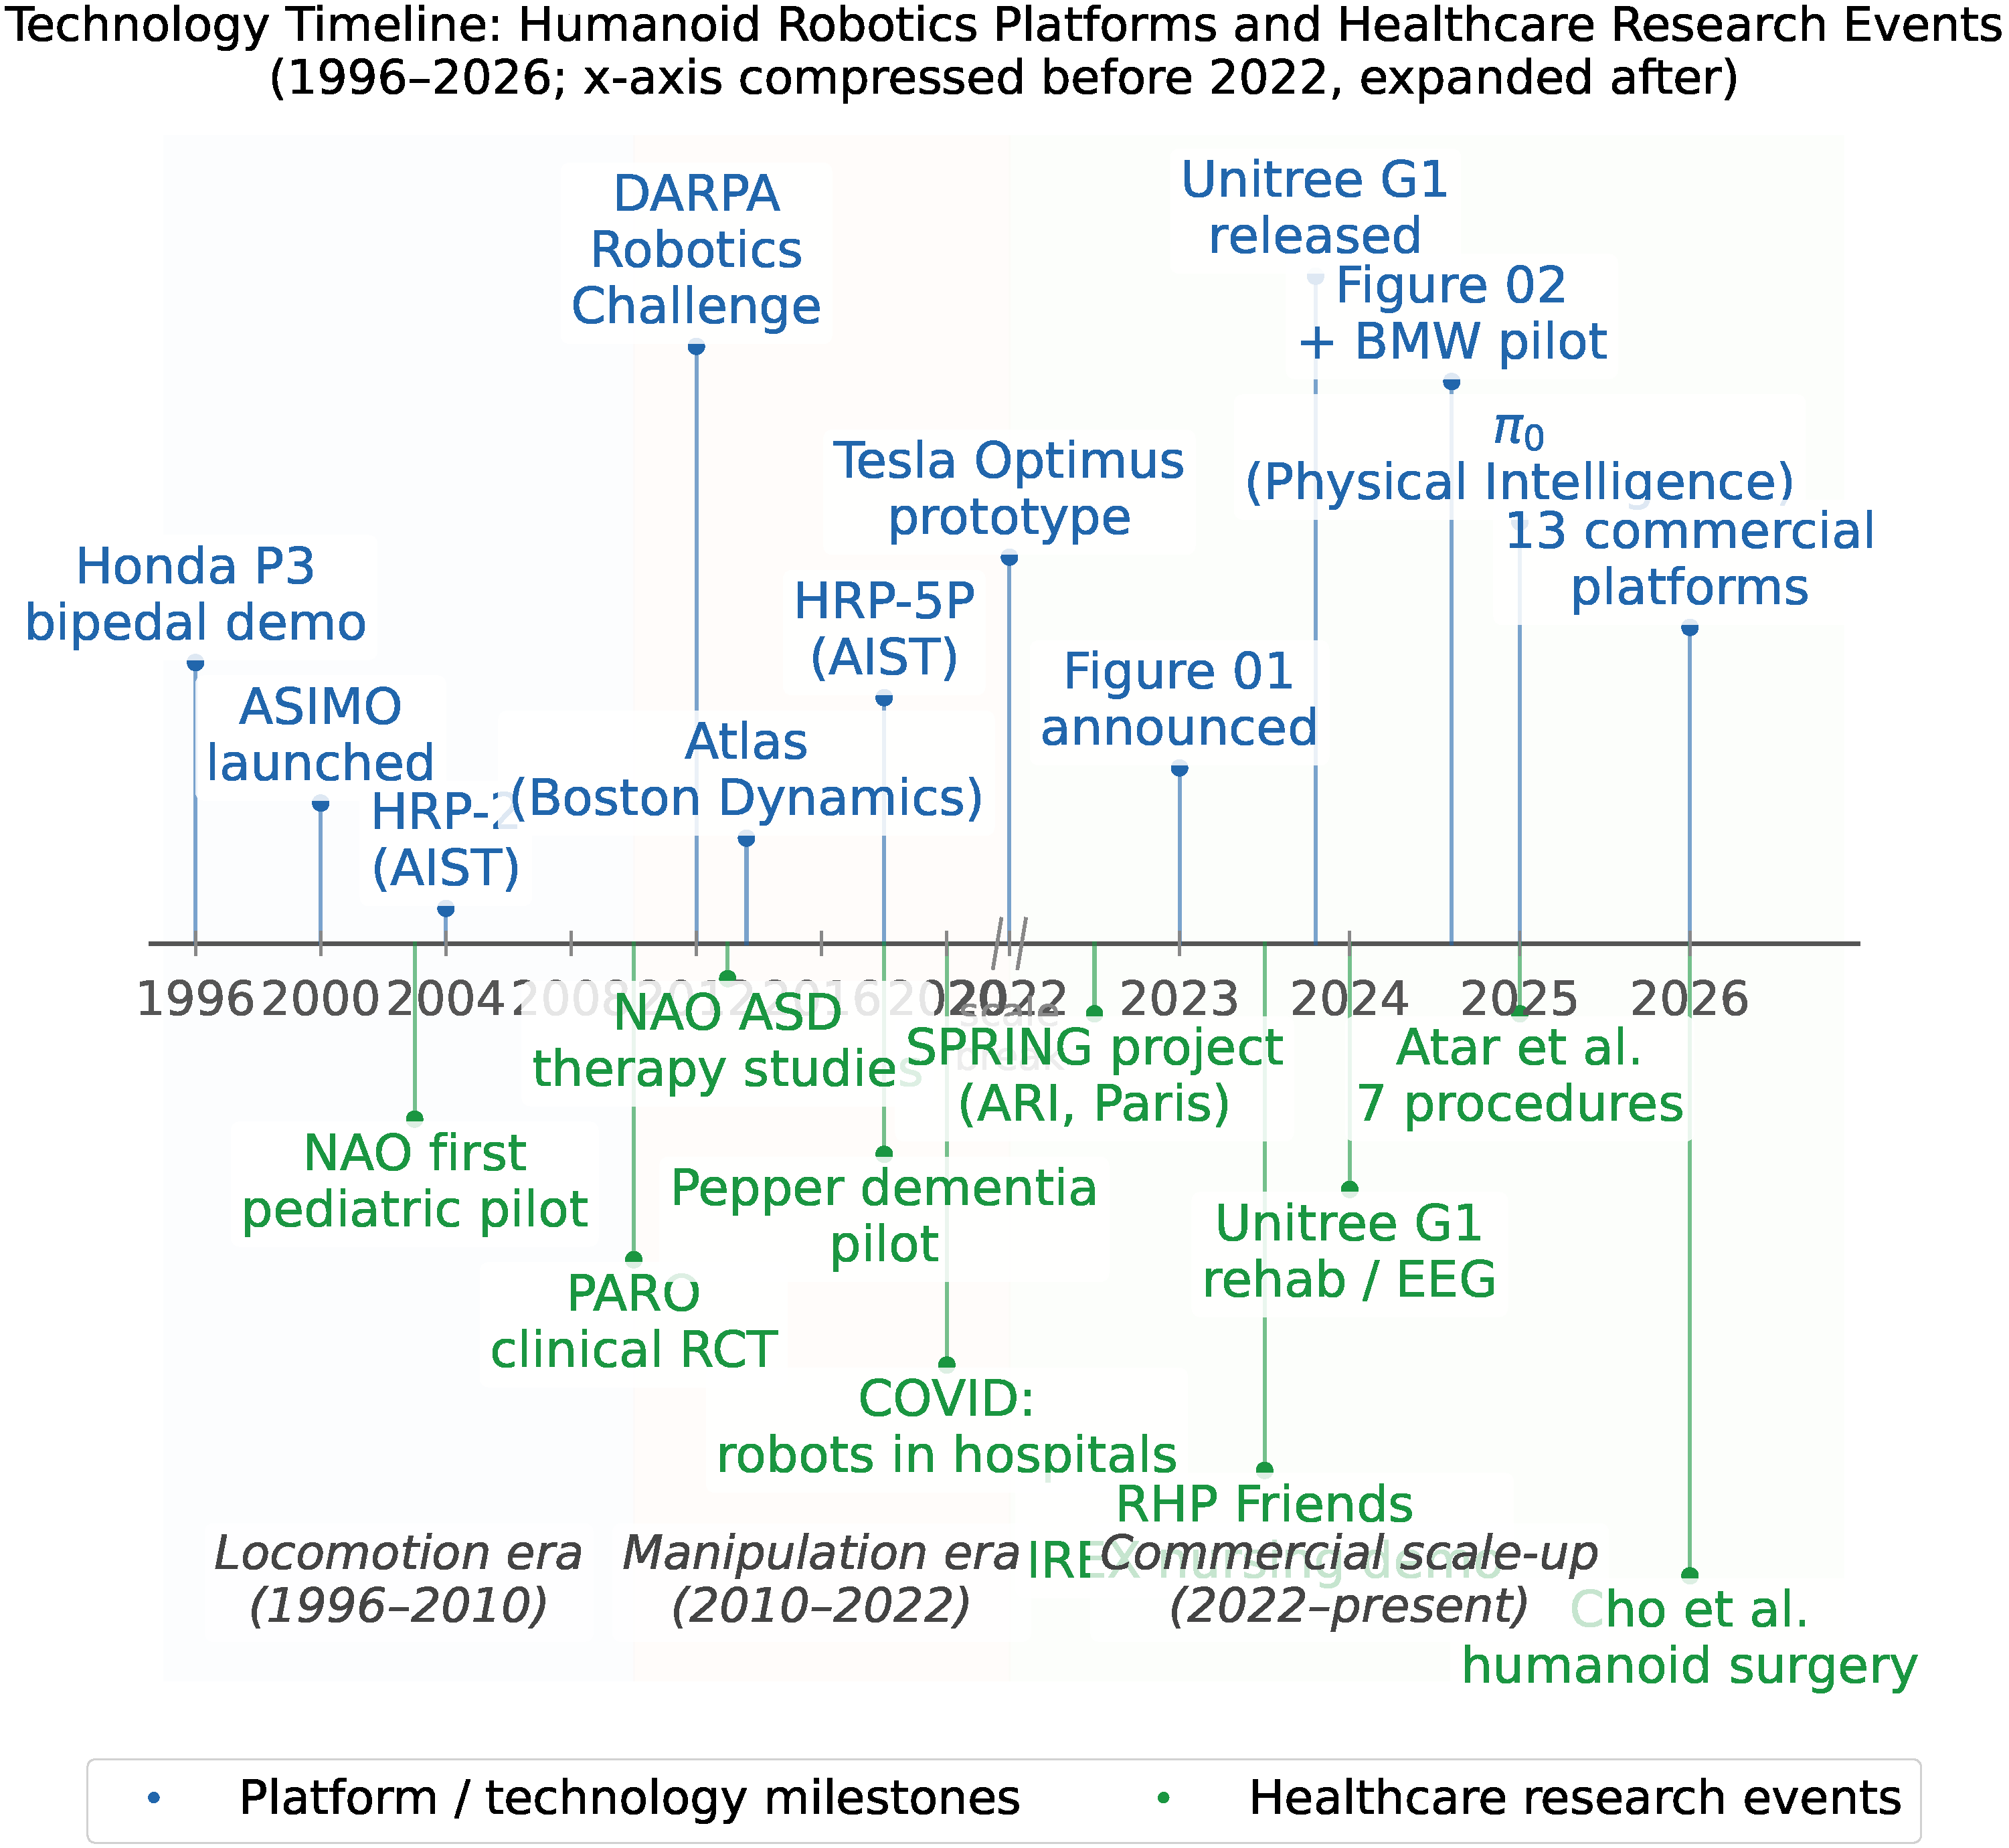
\includegraphics[width=\textwidth]{figures/tech_timeline.pdf}
  \caption{Technology timeline: humanoid robotics platform milestones (upper
  track, blue) and healthcare research events (lower track, green), 1996--2026.
  Shaded regions demarcate three developmental eras: locomotion proof-of-concept
  (1996--2010), manipulation and integration (2010--2022), and commercial
  scale-up (2022--present). Healthcare research events lag platform capability
  by approximately two years in each era.}
  \label{fig:timeline}
\end{figure*}

\subsection{Humanoid Robots vs.\ Non-Humanoid Alternatives in Healthcare}
\label{sec:alternatives}

A principled comparison with existing clinical robot categories is necessary to
locate the humanoid value proposition precisely.

\subsubsection{Social Robots: NAO, Pepper, PARO}

Social robots have the deepest clinical evidence base in robotics. NAO
(SoftBank/Aldebaran, 58~cm, 25~DOF) has accumulated over 1,000 peer-reviewed
publications, with clinical use spanning autism spectrum disorder therapy,
elderly care, and hospital patient reception~\cite{cabibihan2013robots}. Pepper
has been deployed in approximately 2,000 Japanese healthcare facilities for
dementia cognitive stimulation and companion interaction, with embodied
conversational agent frameworks increasingly integrated for clinical
applications~\cite{provoost2017embodied,sorensen2025humanoid,cunha2025humanoid}.
The PARO therapeutic seal robot has demonstrated psychosocial benefits in
randomized controlled trials with elderly residents~\cite{wada2007living}.
These platforms set the deployment high-water mark for robots in clinical care
settings~\cite{abdi2018scoping}. However, their form-factor constraints are real: NAO at 58~cm cannot
reach adult-height work surfaces or perform physical care tasks for adults; Pepper
on a wheeled base cannot navigate stairways or use standard clinical beds.

\subsubsection{Surgical Robots: da~Vinci}

The da~Vinci Surgical System is FDA-cleared (Class~II, 510(k)) with over 10
million procedures completed across urology, gynecology, and general
surgery~\cite{lanfranco2004robotic,sheetz2020robotic}. Robotic surgery adoption
has grown substantially over the past decade, though adverse event analysis
reveals the importance of systematic safety monitoring even for established
platforms~\cite{alemzadeh2016adverse}. The historical trajectory from laboratory
prototype to clinical instrument provides context for humanoid
deployment~\cite{camarillo2004robotic}. Surgical robots are not competitors to
humanoid clinical assistants; they are complementary systems addressing a
fundamentally different need~\cite{morgan2022robots}. Da~Vinci is stationary, surgeon-controlled, and single-purpose.
A humanoid clinical assistant operating in a post-surgical ward addresses the
nursing and logistics tasks that da~Vinci cannot.

\subsubsection{Exoskeletons: ReWalk, HAL, Ekso Bionics}

Wearable robotic exoskeletons are FDA-cleared (Class~II) for spinal cord injury
rehabilitation, with Cochrane-level evidence supporting electromechanical-assisted
training for walking recovery after stroke~\cite{mehrholz2017electromechanical}.
These
rehabilitation~\cite{sorensen2025humanoid}. Exoskeletons assist the patient's own
movement and are not substitutable with a humanoid assistant: they are worn by
the patient, require near-ambulatory capacity, and cannot lift or reposition a
non-ambulatory patient. The GentleHumanoid framework~\cite{lu2025gentlehumanoid}
demonstrates the humanoid's complementary role: learning upper-body compliance
for sit-to-stand assistance addresses patients for whom exoskeletons are not an
option.

\subsubsection{Wheeled Mobile Robots: TUG, Moxi}

Autonomous wheeled mobile robots address hospital logistics with confirmed
operational deployments at major US health systems~\cite{huang2023intelligent,morgan2022robots}.
These systems are purpose-built for point-to-point transport on flat pre-mapped
surfaces. They cannot navigate stairs, interact with clinical equipment not
specifically engineered for their interfaces, or perform physical patient care
tasks. The humanoid argument relative to wheeled logistics robots is a division
of labor argument: wheeled robots solve the logistics layer effectively;
humanoids are needed for the physical assistance and care layer.

\subsection{Section Summary}

The four alternative categories collectively frame a finding that motivates this
review: no existing clinical robot category combines (a)~general ambulatory
mobility in human-built environments, (b)~bimanual dexterous manipulation of
existing clinical tools, and (c)~natural language-mediated task specification
enabling adaptive behavior in unstructured settings. This combination is the
humanoid value proposition for healthcare. The evidence reviewed in this section
characterizes it as \emph{particularly promising}, not as \emph{clinically
proven}. The remainder of this survey characterizes where the field stands, what
has been demonstrated, and what must be resolved before this promise can be
realized.

%%======================================================================
\section{Current Humanoid Systems}
\label{sec:systems}
%%======================================================================

The global humanoid robot landscape in 2024--2026 comprises two largely distinct
populations: commercial platforms designed for industrial labor and a set of
academic research systems whose provenance spans two decades of bipedal
locomotion research. The central empirical finding of this section is that no
confirmed clinical deployment of any full-size bipedal humanoid robot exists as
of March 2026~\cite{atar2025humanoids,cho2026humanoid,cunha2025humanoid}.

\subsection{Commercial Platforms}
\label{sec:commercial}

The commercial humanoid sector underwent a decisive architectural transition
between 2022 and 2024. Earlier systems relied on hydraulic actuation for its high
force density, at the cost of mechanical complexity, fluid-system maintenance,
energy inefficiency, and noise. The generation entering commercial deployment in
2024--2025 is uniformly electric, with brushless DC motors or high-torque servo
actuators. This transition has reduced unit cost, simplified field maintenance,
and enabled quieter operation---properties that are prerequisites for hospital
environments. A second defining characteristic of the 2024--2026 commercial
generation is LLM-native design: twelve of the thirteen systems surveyed were
designed to support VLA models or LLM interfaces for task
specification~\cite{cao2025humanoid}.

\textbf{Tier~1 --- Production-scale deployment.}

\emph{Figure~02} (Figure AI, USA; August 2024) stands at 168~cm and 70~kg, with
28 total degrees of freedom (DOF) and 16~DOF per hand pair. Payload capacity is
20--25~kg; battery runtime is approximately 5~hours. The documented deployment is
a BMW manufacturing facility (Spartanburg, SC), contributing to the assembly of
over 30,000 vehicles over 11 months. No healthcare deployment has occurred.

\emph{Tesla Optimus Gen~2} (Tesla, Inc., USA; December 2023) measures 173~cm and
57~kg, with 28+~body DOF and 11--22 hand DOF. The platform runs Tesla's
Full-Self-Driving-derived neural network stack. Current deployments are internal
to Tesla's factories, performing battery cell sorting and parts handling.
Publicly available documentation does not confirm any clinical deployment or
regulatory submission for medical applications.

\emph{Boston Dynamics Atlas (electric)} (Boston Dynamics/Hyundai Motor Group;
unveiled April 2024) weighs 89~kg with 28~DOF and a sustained payload of 30~kg
(50~kg instantaneous). A strategic partnership with Google DeepMind (announced
CES January 2026) is integrating Gemini Robotics VLA foundation models. Target
deployment is automotive manufacturing. No medical or hospital deployment has
occurred.

\emph{Agility Digit v4} (Agility Robotics/Amazon, USA; commercial deployment
2024) stands 175~cm and 65~kg, with approximately 3~DOF per arm and 16~kg
payload. Confirmed deployments include GXO Logistics (Flowery Branch, GA;
over 100,000 totes moved) and Amazon fulfillment center pilots. Healthcare has
been cited as a long-term target but no clinical deployment has occurred.

\emph{Unitree G1/H1} (Unitree Robotics, China) are the most important commercial
systems for this paper's scope. The H1 (2023) stands 180~cm and 47~kg with
19~DOF; the G1 (May 2024) is 132~cm and 35~kg, with 23--43~DOF (base to EDU
variant), priced at approximately \$13,500--16,000. Unitree is additionally
notable as the only major commercial manufacturer to release and maintain a fully
open-source SDK. The G1 is the \textbf{only commercial humanoid with documented
medical procedure research}: Atar et al.~\cite{atar2025humanoids} at the UC San
Diego Yip Lab demonstrated seven medical procedures with approximately 70\% task
success; Cho et al.~\cite{cho2026humanoid} employed a Unitree G1 as first
assistant in endoscopic surgery. Both constitute academic research prototypes,
not clinical deployments. No Unitree robot has been cleared or deployed as a
clinical tool in any healthcare system.

\textbf{Tier~2 --- Early commercial.}

\emph{1X NEO Beta} (1X Technologies, Norway; August 2024) is the lightest
platform at 30~kg, with 75 total DOF and 22~DOF per hand, noise specified at
22~dB---a potentially relevant characteristic for patient care environments.
\emph{Apptronik Apollo} (Apptronik, USA; August 2023) stands 173~cm and 72.6~kg,
with 25~kg arm payload; current pilots are in automotive assembly (Mercedes-Benz).
\emph{Sanctuary Phoenix Gen~8} (Sanctuary AI, Canada; January 2025) is 170~cm
and 70~kg with 21~DOF per hand and 5~mN tactile force sensitivity---the most
capable haptic sensing in the commercial tier---driven by the proprietary Carbon
AI system developed with Microsoft. No Tier~2 system has a confirmed clinical
deployment.

\textbf{Tier~3 --- Development and pre-commercial.}

\emph{Fourier GR-2} (Fourier Intelligence, China; late 2024) stands 175~cm and
63--65~kg with 53 total DOF and 12 hand DOF per pair, with six tactile sensor
arrays. Fourier Intelligence has a healthcare-affiliated subsidiary with
confirmed research collaborations at Shirley Ryan AbilityLab and Tan Tock Seng
Hospital; however, these partnerships involve exoskeleton devices, not the GR-2
humanoid. \emph{UBTECH Walker~X} (UBTECH Robotics, China) is 130--145~cm and
63--77~kg with 41~DOF and multimodal LLM integration; UBTECH maintains a
separate healthcare product line distinct from Walker~X. \emph{AgiBot A2}
(AgiBot/Zhiyuan, China; 2024) is 175~cm and 55~kg with 49+~DOF and an estimated
5,168 units shipped in 2025 (all industrial and service contexts). \emph{NEURA
4NE-1} (NEURA Robotics, Germany; 2023--2024) is 170--180~cm with confirmed
force-torque sensing at 0.1~N sensitivity. No Tier~3 system has a confirmed
clinical deployment.

\textbf{Deployment reality.} All thirteen commercial systems surveyed are
deployed exclusively in industrial or logistics contexts as of March 2026. The
sole departure from this pattern is the Unitree G1's use as a research prototype
in two academic medical studies~\cite{atar2025humanoids,cho2026humanoid}. The gap
between demonstrated capability in controlled industrial tasks and validated
safety in patient-contact clinical environments remains the central barrier to
medical deployment.

\subsection{Academic and Research Platforms}
\label{sec:academic}

\textbf{RHP Friends} (CNRS-AIST Joint Robotics Laboratory/Kawasaki Heavy
Industries, Japan/France) is the only academic humanoid explicitly designed and
demonstrated for nursing care~\cite{benallegue2025rhp}. At 168~cm and 54~kg with
30~DOF, it is human-scale and directly deployable in standard clinical
environments. Its defining architectural feature is seamless switching between
autonomous and teleoperated control: routine tasks execute autonomously while
non-routine or high-stakes tasks hand off to a remote human operator without
observable interruption. The system was demonstrated at IREX 2023 over three days
executing patient transfer assistance and circuit breaker operation. No patients
were involved. This constitutes the most directly healthcare-relevant academic
humanoid performance documented in the literature.

\textbf{NAO} (Aldebaran Robotics/SoftBank Robotics; V6 current) is the most
extensively studied humanoid in healthcare research (over 1,000 peer-reviewed
publications). At 58~cm and 5.6~kg with 25~DOF, it has been deployed in ASD
therapy trials, elderly care facilities, and hospital waiting areas. Over 19,000
units are distributed globally. \emph{Scope caveat}: NAO's form factor is
categorically unsuitable for physical adult care tasks. All clinical evidence for
NAO pertains to social and cognitive interaction.

\textbf{Pepper} (SoftBank Robotics/Aldebaran) is the most extensively deployed
humanoid-form robot in operational healthcare settings: over 2,000 Japanese care
facilities use or have used Pepper for dementia cognitive stimulation and
companion interaction. Production was paused in June 2021. \emph{Scope caveat}:
Pepper is 120~cm and moves on a three-wheeled omnidirectional base---it is not
bipedal and does not meet this paper's scope definition.

\textbf{iCub/iCub3} (Italian Institute of Technology; 2004--present) is 104~cm
and approximately 23~kg with 54~DOF and full-body capacitive tactile skin. iCub3
(2022) adds immersive telepresence capability. Over 40 units are distributed to
research laboratories worldwide. No confirmed clinical deployment exists.
Platforms without confirmed healthcare use include TALOS (PAL Robotics), Valkyrie
(NASA JSC), WALK-MAN (IIT), TORO (DLR), LOLA (TU Munich), and the discontinued
ASIMO (Honda, retired 2022).

\subsection{Capability Comparison}
\label{sec:comparison}

Table~\ref{tab:platforms} compares key specifications for all commercial and
selected academic humanoid platforms. All values are drawn directly from verified
primary sources; unknown or undisclosed values are marked N/A; approximate values
are prefixed with $\sim$. The Medical Deployment column reflects confirmed
deployments only.

\begin{table*}[t]
  \caption{Humanoid Platform Capability Comparison (March 2026). N/A = not
  publicly disclosed. \textsuperscript{$\dagger$}Research prototype only, not
  clinical deployment. \textsuperscript{*}Not bipedal under this paper's scope
  definition; included as deployment benchmark.}
  \label{tab:platforms}
  \resizebox{\linewidth}{!}{%
  \begin{tabular}{@{}llrllllll@{}}
    \toprule
    \textbf{Robot} & \textbf{Type} & \textbf{Ht} &
    \textbf{Arm DOF} & \textbf{Payload} &
    \textbf{LLM Integration} & \textbf{Open SW} &
    \textbf{Medical Deployment} \\
    \midrule
    Figure 02        & Commercial & 168 & N/A (28 total) & 20--25\,kg & Yes (in-house VLA)    & No      & None \\
    Tesla Optimus G2 & Commercial & 173 & N/A (28+ total)& 20\,kg     & Yes (FSD-derived)     & No      & None \\
    BD Atlas (elec.) & Commercial & $\sim$165 & N/A (28 total) & 30\,kg & Yes (Gemini, announced) & No & None \\
    Agility Digit v4 & Commercial & 175 & $\sim$3/arm    & 16\,kg     & Announced             & Partial & None \\
    Unitree G1       & Commercial & 132 & N/A (23--43)   & N/A        & Yes (VLA, open)       & Yes     & Research proto.~\cite{atar2025humanoids,cho2026humanoid}\textsuperscript{$\dagger$} \\
    Unitree H1       & Commercial & 180 & N/A (19 total) & N/A        & Yes (open)            & Yes     & None \\
    1X NEO Beta      & Commercial & 165 & 22/hand        & 25\,kg     & Yes (proprietary)     & No      & None \\
    Apptronik Apollo & Commercial & 173 & N/A            & 25\,kg     & Yes (Google AI)       & No      & None \\
    Sanctuary Ph. G8 & Commercial & 170 & 21/hand        & 25\,kg     & Yes (Carbon/Microsoft)& No      & None \\
    Fourier GR-2     & Commercial & 175 & 12/arm pair    & N/A        & Announced             & Partial & None \\
    UBTECH Walker X  & Commercial & 130--145 & 7/arm      & 10\,kg    & Yes (multimodal LLM)  & No      & None \\
    AgiBot A2        & Commercial & 175 & 7/arm          & N/A        & Yes (proprietary)     & No      & None \\
    NEURA 4NE-1      & Commercial & $\sim$175 & N/A       & 15--20\,kg & Yes (cognitive AI)   & No      & None \\
    RHP Friends      & Academic   & 168 & 7/arm          & N/A        & No                    & Partial & IREX 2023 nursing demo~\cite{benallegue2025rhp} \\
    NAO\textsuperscript{*} & Academic & 58 & N/A (25 total) & N/A   & No                    & Partial & HRI/ASD trials (social only) \\
    Pepper\textsuperscript{*} & Academic & 120 & N/A    & N/A        & No                    & Partial & 2,000+ Japan care facilities \\
    \bottomrule
  \end{tabular}%
  }
\end{table*}

\subsection{Open-Source Software Ecosystem}
\label{sec:opensource}

A survey of prominent open-source repositories relevant to humanoid robotics
yields a clear finding: no dedicated software stack exists for humanoid medical
deployment. What does exist is a maturing ecosystem of general-purpose
infrastructure.

\textbf{Foundation models and VLA frameworks.} LeRobot~\cite{cadene2024lerobot}
(HuggingFace; 22,179~stars; Apache~2.0) provides a standardized, hardware-agnostic
pipeline for training imitation learning and VLA policies with direct hardware
support for the Unitree G1. Physical Intelligence's openpi provides the
$\pi_0$~\cite{black2024pi0} VLA foundation model pre-trained on over 10,000~hours
of real robot demonstrations, with state-of-the-art results on ALOHA bimanual
manipulation benchmarks~\cite{zhao2023act} and support for fine-tuning with
minimal demonstrations. OpenVLA~\cite{kim2024openvla} (openvla/openvla;
5,479~stars; MIT), a collaboration of Stanford, Berkeley, and Toyota Research
Institute, is a 7B-parameter VLA model trained on 970,000 real-world demonstrations
from the Open X-Embodiment dataset~\cite{openxembodiment2023}. The Diffusion
Policy~\cite{chi2023diffusion} framework provides a complementary visuomotor
policy approach based on denoising diffusion models. All four are general-purpose
manipulation frameworks with no healthcare-specific training data, safety
validation, or clinical task benchmarks.

\textbf{Simulation environments.} Genesis (Genesis-Embodied-AI/Genesis;
28,254~stars; Apache~2.0) is a unified differentiable physics simulation platform
released in December 2024. Isaac Lab (isaac-sim/IsaacLab; 6,544~stars;
BSD-3-Clause) is NVIDIA's GPU-accelerated framework with direct support for
Unitree G1 and H1. Neither platform provides medical environment models, clinical
workflow scenarios, or validated patient-contact physics.

\textbf{Unitree hardware ecosystem.} The Unitree GitHub organization maintains
nine publicly accessible repositories including unitree\_rl\_gym (3,022~stars),
unitree\_sdk2 (932~stars), and xr\_teleoperate (1,309~stars) for full-body
teleoperation via XR headsets---the software component used in the Atar et
al.\ teleoperation study~\cite{atar2025humanoids}.

\textbf{The infrastructure gap.} Four categories of infrastructure required for
clinical deployment are entirely absent from the open-source ecosystem: (1)~a
validated safety layer enforcing patient-contact force limits at runtime;
(2)~clinical workflow integration connecting humanoid actions to hospital EHR and
nursing systems; (3)~an open clinical demonstration dataset (every major VLA
training corpus consists of household and tabletop tasks); and (4)~a validated
medical simulation environment with clinical instrument physics and patient
anatomy proxies. The transition from ``general-purpose manipulation capability''
to ``clinically safe, task-verified medical assistance'' is primarily a software
and validation challenge for which the open-source community has not yet produced
foundational components.

Table~\ref{tab:opensource} summarizes the most prominent open-source repositories
in this ecosystem.

\begin{table*}[t]
  \caption{Open-Source Software Ecosystem for Humanoid and Embodied-AI Robotics
  (March 2026). Stars are approximate GitHub counts at time of writing. Medical
  Relevance: \textbf{H}~=~high (direct hardware/algorithm support for clinical
  candidate platforms), \textbf{M}~=~medium (transferable general capability),
  \textbf{L}~=~low (infrastructure/simulation only). No repository provides
  clinical-specific safety validation or medical workflow integration.}
  \label{tab:opensource}
  \resizebox{\linewidth}{!}{%
  \begin{tabular}{@{}llrllp{4.5cm}l@{}}
    \toprule
    \textbf{Repository} & \textbf{Org / Author} & \textbf{Stars} &
    \textbf{Purpose} & \textbf{License} & \textbf{Notes} & \textbf{Med.\ Rel.} \\
    \midrule
    lerobot            & HuggingFace        & $\sim$22k  & VLA/imitation learning pipeline  & Apache 2.0  & Supports Unitree G1; no clinical data & H \\
    openpi             & Physical Intelligence & $\sim$10k & $\pi_0$ VLA foundation model      & Apache 2.0  & 10k+ hrs robot demos; bimanual ALOHA   & H \\
    openvla            & Stanford/Berkeley/TRI & $\sim$5.4k & 7B-param open VLA model          & MIT         & 970k demos; generalist manipulation    & H \\
    act                & tonyzhaozh         & $\sim$5k   & Action Chunking Transformers      & MIT         & Original ALOHA bimanual policy code    & H \\
    diffusion\_policy  & Columbia/MIT       & $\sim$4.5k & Diffusion-based robot policy      & MIT         & State-of-art imitation learning        & M \\
    Genesis            & Genesis-Embodied-AI & $\sim$28k & Differentiable physics simulation & Apache 2.0  & No medical environment models          & M \\
    IsaacLab           & isaac-sim (NVIDIA) & $\sim$6.5k & GPU-accelerated RL + sim          & BSD-3       & G1/H1 native support; no clinical env. & M \\
    unitree\_rl\_gym   & Unitree Robotics   & $\sim$3k   & RL locomotion for Unitree robots   & BSD-3       & G1/H1/B2 locomotion training           & H \\
    xr\_teleoperate    & Unitree Robotics   & $\sim$1.3k & Full-body XR teleoperation        & Apache 2.0  & Used in Atar et al.\ 2025 study        & H \\
    unitree\_sdk2      & Unitree Robotics   & $\sim$0.9k & Hardware SDK for G1/H1/B2         & Apache 2.0  & Low-level hardware interface           & H \\
    ManiSkill          & HKUST              & $\sim$1.8k & Embodied manipulation benchmark   & Apache 2.0  & No clinical task benchmarks            & M \\
    RoboManip          & isri-robot         & $\sim$0.3k & Bimanual manipulation dataset     & MIT         & Tabletop tasks only                    & M \\
    Open Duck Mini     & apirrone           & $\sim$2k   & Miniature bipedal robot (open HW) & MIT         & Educational; not clinical scale        & L \\
    \midrule
    \multicolumn{7}{@{}l}{\emph{Medical infrastructure (absent from ecosystem)}} \\
    \midrule
    (none)             & ---                & ---        & Clinical safety layer (PFL/gait)  & ---         & No validated implementation exists     & --- \\
    (none)             & ---                & ---        & Medical simulation environment    & ---         & No clinical instrument/anatomy physics & --- \\
    (none)             & ---                & ---        & Open clinical demonstration data  & ---         & All major VLA datasets are non-medical & --- \\
    \bottomrule
  \end{tabular}%
  }
\end{table*}

%%======================================================================
\section{Medical Applications and Research}
\label{sec:applications}
%%======================================================================

Despite growing interest in humanoid robots for healthcare, the peer-reviewed
evidence base as of early 2026 is remarkably sparse. A systematic search spanning
arXiv, PubMed, IEEE Xplore, ACM Digital Library, and Google Scholar, covering
2022--2026, yielded 14 qualifying papers under the bipedal-or-human-form humanoid
scope defined in Section~\ref{sec:background}. The literature is strongly
concentrated on a single commercial platform---the Unitree G1---and is dominated
by a single research cluster (the UC San Diego Yip Laboratory and Johns Hopkins
University), which together account for all three papers in the clinical
procedures domain. This concentration is itself a finding: the evidence for
humanoid robot capability in clinical settings is real but narrow, and
independent replication on alternative platforms has not yet occurred.

\subsection{Clinical Procedures and Surgical Assistance}
\label{sec:procedures}

The most substantive cluster of evidence concerns teleoperated humanoid robots
performing discrete clinical procedures. Three papers constitute this cluster,
all published between 2025 and 2026, all using the Unitree G1.

\textbf{Bimanual teleoperation for dexterous medical interventions.} Atar et
al.~\cite{atar2025humanoids} (UC San Diego Yip Laboratory, PI: Michael Yip)
developed a bimanual teleoperation system integrating the Unitree G1 with Inspire
Gen4 dexterous hands---four-fingered grippers with 12~DOF each---controlled via
bilateral impedance control and real-time motion retargeting. The system was
evaluated across seven distinct clinical procedures: (1)~cardiac and pulmonary
auscultation via stethoscope placement, (2)~respiratory assistance via bag-valve
mask ventilation, (3)~Leopold maneuvers for fetal position assessment,
(4)~otoscopic examination, (5)~intravenous catheter insertion, (6)~point-of-care
ultrasound (POCUS), and (7)~blood glucose finger-stick testing. Non-clinician
operators achieved an aggregate procedural success rate of approximately 70\% in
controlled laboratory conditions; no human subjects were involved. Auscultation
and ultrasound imaging yielded the strongest performance; IV catheter insertion
and finger-stick testing were the most challenging, with failures attributable to
force precision requirements beyond the system's current capability.

The paper documents two technical barriers: insufficient force output in the
actuator configuration, and sensor sensitivity limitations in the tactile
feedback loop. The study is assessed at TRL~4---technology validated in laboratory
conditions using representative test fixtures, but not yet in a clinical
environment or with patient contact.

\textbf{Laparoscopic surgery via humanoid teleoperation.} Liang et
al.~\cite{liang2025lapsurgie} (UCSD Yip Laboratory) extend humanoid clinical
teleoperation to laparoscopic surgery. Their LapSurgie framework introduces an
inverse-mapping strategy adapting the Unitree G1's arm kinematics to drive
manual-wristed laparoscopic instruments while enforcing a remote-center-of-motion
(RCM) constraint at the trocar site---a non-negotiable geometric safety
requirement ensuring the instrument pivots about the entry point rather than
exerting lateral forces on the abdominal wall. The authors advance an
access-equity argument: the humanoid form factor maps naturally to laparoscopic
ergonomic conventions, potentially enabling specialist surgical capability in
geographically underserved settings.

\textbf{Humanoid robot as surgical first assistant.} Cho et
al.~\cite{cho2026humanoid} (Johns Hopkins University) report the most clinically
significant result in this review: a teleoperated Unitree G1 serving as first
assistant in a bilateral cadaveric sphenoidectomy performed by an attending
otolaryngologist. The robot held and repositioned an endoscope under the
surgeon's direction, providing the continuous endoscopic visualization that a
human first assistant would normally supply. This is the first documented use of
a modern commercial bipedal humanoid in a real surgical procedural context.
Cadaver studies are a recognized pre-clinical methodology representing the step
immediately preceding IRB protocols with human subjects. The paper identifies
specific engineering targets for clinical translation: endoscope stability,
compliant force control during anatomical contact, and autonomous scope
positioning.

\textbf{Platform concentration as a structural limitation.} All three papers in
this subsection use the Unitree G1; P1 and P2 originate from a single laboratory
under a single principal investigator. Independent replication on other platforms
has not yet occurred, limiting generalizability of the current evidence base.

\subsection{Elderly and Nursing Care}
\label{sec:eldercare}

\textbf{Purpose-built nursing humanoid.} Benallegue et
al.~\cite{benallegue2025rhp} document RHP Friends, the only bipedal humanoid
platform in the literature designed with nursing assistance as its explicit
primary application. Its defining architectural contribution is seamless
transparent switching between autonomous and teleoperated control: routine tasks
execute autonomously while non-routine tasks hand off to a remote human operator
without observable interruption. The system was demonstrated at IREX 2023
performing patient transfer assistance and circuit breaker operation. No patients
were involved. TRL~4 for demonstrated hardware capability in a structured
exhibition setting.

\textbf{Large-scale deployment evidence from a wheeled platform.}
\emph{Scope caveat}: the SPRING project~\cite{alamedapineda2024spring} used the
ARI robot by PAL Robotics, which operates on a wheeled differential-drive base;
it does not qualify as a bipedal humanoid and must not be cited as evidence for
bipedal humanoid deployment. Over a four-year EU H2020 program (2020--2024), ARI
was deployed in a Parisian geriatric day-care facility with more than 60 older
adult participants. Acceptability was positive; participants specifically cited
upright posture and eye-level conversational positioning as important for
dignified interaction. The SPRING project represents the deployment robustness
and user acceptance threshold that fully bipedal systems must replicate.

\textbf{Institutional stakeholder perspectives.} Imtiaz and
Khan~\cite{imtiaz2024perceptions} surveyed 269 nursing home and long-term care
administrators across the United States on humanoid robot deployment. Administrators
acknowledged potential value in resident engagement and staff support. Primary
barriers cited were cost, perceived risk of reduced human contact, and the absence
of demonstrated clinical effectiveness data---objections that are economic,
ethical, and evidence-based rather than technical.

\textbf{User-centered design methodology.} Ghosh et
al.~\cite{ghosh2024usercentered} report a user-centered design study combining a
NAO humanoid with non-immersive virtual reality for non-pharmacological apathy
management (14 participants). \emph{Scope caveat}: NAO is 58~cm and not a
full-size bipedal humanoid. The study's contribution is methodological:
iterative co-design with care staff improved system usability across design
cycles, demonstrating that clinical staff can be engaged as design partners.

\subsection{Rehabilitation}
\label{sec:rehabilitation}

\textbf{Neuroscientific basis for humanoid-specific rehabilitation.} Nguyen,
Anand, and Johnson~\cite{nguyen2024eeg} report a pilot EEG study measuring
sensorimotor neural responses in healthy participants during observation of a
humanoid robot versus a human actor performing reaching and grasping actions. The
central finding is that common neural response patterns consistent with mirror
neuron system activation are elicited by humanoid robot observation at levels
comparable to human observation. This is a foundational result for the use of
humanoid robots as movement demonstrators in AOT programs for stroke patients.
Caveats: pilot study in healthy subjects; clinical replication in patients with
motor impairment is necessary. TRL: 3 (experimental proof of concept).

\textbf{Remote neuromotor rehabilitation via humanoid telepresence.} Sobrepera
et al.~\cite{sobrepera2022feasibility} describe a Social Robot Augmented
Telepresence (SRAT) system combining a humanoid robot with mobile telepresence
for remote neuromotor rehabilitation. A case series of six participants (three
adult stroke survivors, three pediatric participants) found that five of six rated
the SRAT system superior to standard video telepresence, attributing the
preference to the physical embodiment of the humanoid---the ability to
demonstrate movement and convey nonverbal cues through body posture. TRL: 4,
demonstrated in a small clinical case series.

\textbf{Compliance for physical assistance tasks.} Lu et
al.~\cite{lu2025gentlehumanoid} report the GentleHumanoid framework, a
spring-based unified compliance architecture for the Unitree G1 enabling safe
physical contact during sit-to-stand assistance and upper-body interactions. No
patient subjects were involved. The framework's quantified reduction in peak
contact forces relative to rigid control constitutes a concrete step toward the
force limits specified by ISO/TS~15066 for physical human-robot contact.

\subsection{Mental Health and Social Interaction}
\label{sec:mentalhealth}

\textbf{Autonomous humanoid delivery of wellbeing intervention.} Robinson et
al.~\cite{robinson2023brief} report a pilot randomized controlled trial
(n\,=\,230) in which an autonomous humanoid social robot delivered a brief
mindful breathing training session to a subclinical general population.
Recruitment uptake of 53\% indicates the intervention was not aversive.
Participants rated the experience as enjoyable and moderately useful. \emph{Caveat}:
subclinical general population; robot model undisclosed; primary measure was
self-reported experience. TRL: 4 for wellbeing applications in non-clinical
settings.

\textbf{Embodiment advantage in mental health interactions.} Sayis and
Gunes~\cite{sayis2024technology} report a comparative study (n\,=\,42 university
students) of humanoid robot versus voice assistant for therapeutic journal
writing. Only the humanoid robot condition produced statistically significant mood
improvements, increased self-disclosure, and positive perception change.
\emph{Caveat}: university wellness population; robot model unspecified. The
embodiment advantage finding merits replication in clinical populations.

\textbf{LLM integration for personalized dementia care.} Yuan et
al.~\cite{yuan2025integrating} propose a framework combining a humanoid robot,
reinforcement learning, and large language models for adaptive personalized
dementia care, introducing probabilistic cognitive-emotional state modeling.
\emph{Scope caveat}: this paper uses Pepper, a wheeled robot. It is cited here
exclusively for the LLM integration paradigm---cognitive-emotional state modeling
adaptable to bipedal platforms. The use of embodied conversational agents for
clinical psychology applications is a growing evidence base~\cite{provoost2017embodied}.

Socially assistive robots with automated planning have also been explored in
paediatric clinical settings~\cite{lindsay2022socially}, providing methodological
precedent for structured social robot interaction protocols.

\subsection{Hospital Logistics}
\label{sec:logistics}

No qualifying papers were found for humanoid-specific hospital logistics tasks
performed by bipedal humanoid robots. This absence is plausibly explained by two
structural factors. First, wheeled autonomous mobile robots already address
hospital logistics with proven operational reliability, providing no demonstrated
functional advantage for the humanoid form factor in this task category. Second,
humanoid hardware development in 2022--2026 was concentrated on high-value
industrial contexts, with academic research attention directed toward the more
scientifically novel clinical procedure and HRI domains. TRL for bipedal humanoid
hospital logistics: 2 (technology concept formulated; no demonstrated examples in
relevant contexts).

\subsection{Section Summary}
\label{sec:appsummary}

Table~\ref{tab:evidence} summarizes the evidence base across the five clinical
domains reviewed above.

\begin{table}[t]
  \caption{Evidence Summary by Clinical Domain (as of March 2026). TRL per ISO
  16290:2013: 1\,=\,basic principles; 2\,=\,concept formulated;
  3\,=\,experimental PoC; 4\,=\,lab validated; 5\,=\,relevant-environment
  validated; 7\,=\,operational prototype; 9\,=\,proven.
  \textsuperscript{*}ARI/SPRING: wheeled platform, not bipedal; scope caveat applies.}
  \label{tab:evidence}
  \footnotesize
  \begin{tabular}{@{}p{2.1cm}p{2.1cm}p{2.0cm}p{1.4cm}p{1.1cm}l@{}}
    \toprule
    \textbf{Domain} & \textbf{Key Papers} & \textbf{Platform} & \textbf{Study Type} & \textbf{N} & \textbf{TRL} \\
    \midrule
    Clinical procedures &
      P1~\cite{atar2025humanoids}, P2~\cite{liang2025lapsurgie}, P3~\cite{cho2026humanoid} &
      Unitree G1 & Lab; user study; cadaver & 0 patients & 3--4 \\[3pt]
    Elderly / nursing &
      P8~\cite{benallegue2025rhp}, P7\textsuperscript{*}~\cite{alamedapineda2024spring} &
      RHP Friends; ARI\textsuperscript{*} & Exhibition demo; field deploy. &
      0 (demo); 60+\textsuperscript{*} & 4; 4--5\textsuperscript{*} \\[3pt]
    Rehabilitation &
      P5~\cite{nguyen2024eeg}, P6~\cite{sobrepera2022feasibility}, P13~\cite{lu2025gentlehumanoid} &
      Humanoid; SRAT; Unitree G1 & EEG pilot; case series; engineering &
      0 / 6 / 0 & 3--4 \\[3pt]
    Mental health / HRI &
      P11~\cite{robinson2023brief}, P14~\cite{sayis2024technology} &
      Unspecified humanoid & RCT; comparative & 230; 42 & 4--5 \\[3pt]
    Hospital logistics & --- & --- & None & --- & 2 \\
    \bottomrule
  \end{tabular}
\end{table}

The aggregate picture across all five domains is consistent: the field is at
TRL~3--4 for bipedal humanoid clinical tasks. Feasibility has been demonstrated
in controlled laboratory and pre-clinical settings, primarily by two research
groups on a single platform, but no clinical trial with patient subjects, no
regulatory submission, and no institutional deployment exists for any full-size
bipedal humanoid robot as of early 2026.

Figure~\ref{fig:landscape} visualizes the distribution of the 14 qualifying
papers by domain and year, with bubble size proportional to study design strength.

\begin{figure*}[t]
  \centering
  \Description{Scatter plot showing 14 qualifying papers organized by clinical
  domain (y-axis: Clinical Procedures, Elderly/Nursing Care, Rehabilitation,
  Mental Health/HRI) and publication year (x-axis: 2022-2026). Bubble size is
  proportional to study design strength: RCT and case series are larger than
  engineering and pilot studies. Clinical procedure papers are concentrated
  in 2025-2026; mental health studies span 2023-2025; rehabilitation studies
  span 2022-2025; elderly/nursing care studies span 2022-2025.}
  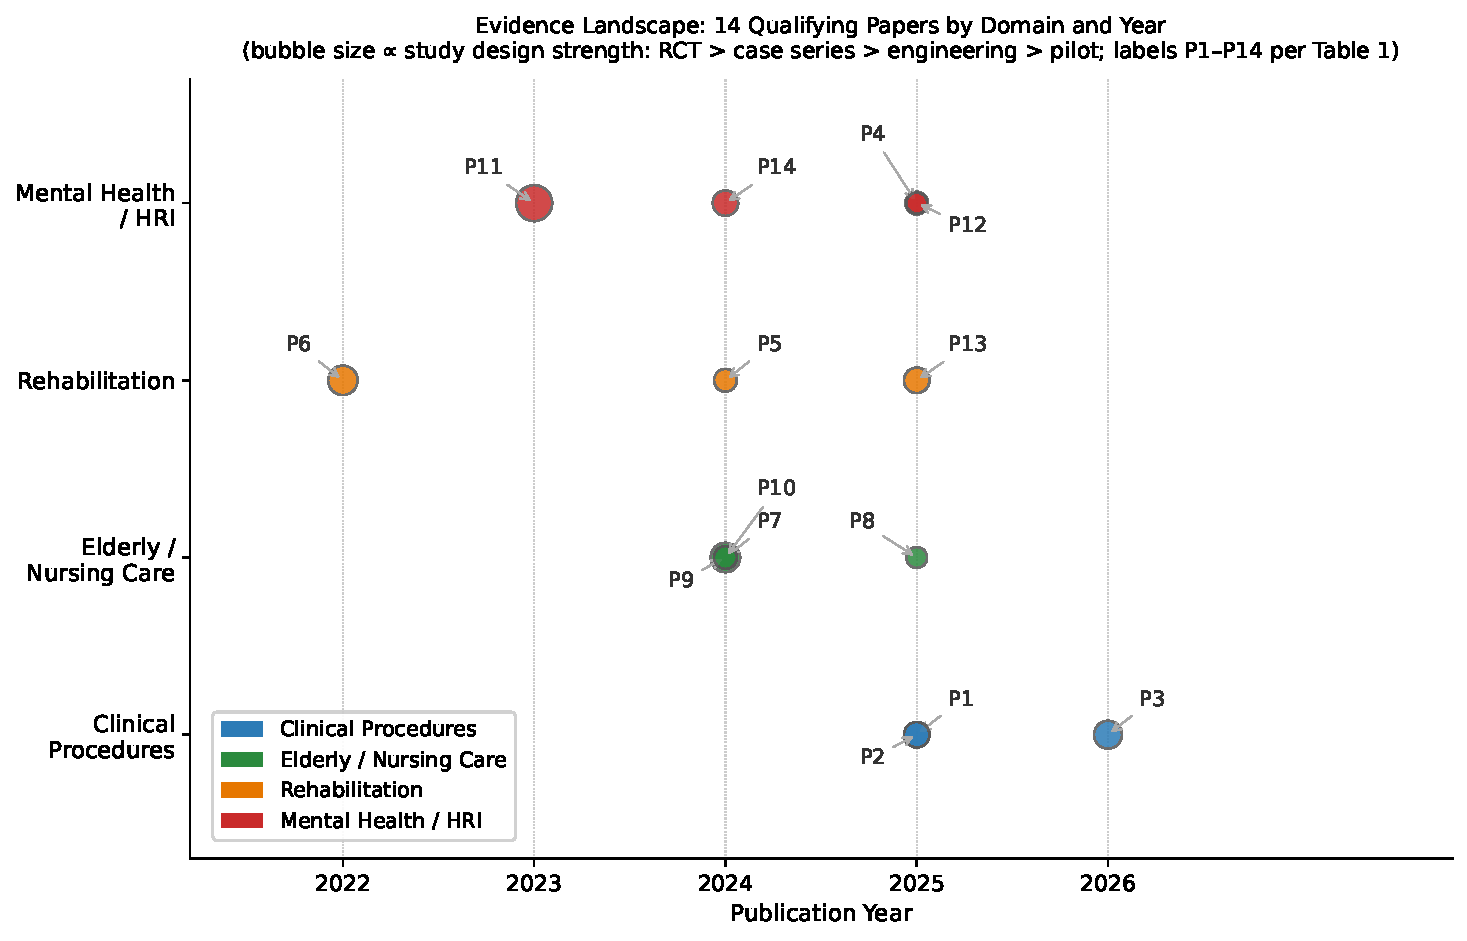
\includegraphics[width=\textwidth]{figures/evidence_landscape.pdf}
  \caption{Evidence landscape: 14 qualifying papers by clinical domain and
  publication year (bubble size proportional to study design strength:
  RCT\,$>$\,case series\,$>$\,engineering\,$>$\,pilot). Clinical procedure
  evidence (blue) is concentrated in 2025--2026 and from a single platform and
  research cluster. Rehabilitation (orange) and mental health (red) evidence is
  more temporally distributed but also methodologically limited. No papers qualify
  for hospital logistics.}
  \label{fig:landscape}
\end{figure*}

%%======================================================================
\section{Technical and Translational Challenges}
\label{sec:challenges}
%%======================================================================

The TRL~3--4 state documented in Section~\ref{sec:applications} reflects a
specific constellation of barriers that are neither uniform nor independently
solvable. Some are technical: manipulation precision, contact safety during
bipedal locomotion, software validation against clinical performance standards.
Some are institutional: regulatory pathway ambiguity, liability framework gaps,
actuarial absence. And some are structurally circular: regulatory approval
requires clinical evidence; clinical evidence requires IRB-sanctioned trials; IRB
approval requires safety assurance; safety assurance requires performance
standards that regulatory guidance has not yet established. This section diagnoses
each barrier specifically.

\subsection{Manipulation and Dexterity for Clinical Tools}
\label{sec:manipulation}

Atar et al.~\cite{atar2025humanoids} is the only study to systematically document
manipulation performance gaps in a clinical task context. Atar et al.\ evaluated
a Unitree G1 with Inspire Gen4 dexterous hands across seven clinical procedures,
achieving approximately 70\% aggregate procedural success with non-clinician
teleoperators. The paper identifies two specific failure modes: force output
insufficiency (the actuator configuration cannot reliably generate the controlled
forces required for needle penetration or sustained grip against resistance), and
sensor sensitivity limitations (the tactile feedback loop is insufficient for
sub-Newton force resolution, preventing detection of the haptic signatures that
guide needle procedures in clinical practice).

These findings generalize across the procedure literature. Liang et
al.~\cite{liang2025lapsurgie} demonstrate that laparoscopic surgery requires
enforcing a remote-center-of-motion (RCM) constraint at the trocar site---an
engineering workaround for a capability that commercial humanoid arms do not
provide natively. Cho et al.~\cite{cho2026humanoid} identify three engineering
targets for endoscopic clinical translation: endoscope stability in confined
anatomical cavities, force compliance during tissue contact, and positioning
accuracy for reliable camera view.

Synthesizing across P1, P2, and P3, clinical manipulation requires three
capabilities that current commercial humanoid arms do not yet reliably provide:
(1)~force precision at sub-Newton resolution for needle and catheter
procedures~\cite{atar2025humanoids}; (2)~tool-specific kinematic adaptation for
laparoscopes, rigid endoscopes, and ultrasound probes; and (3)~fingertip-level
tactile sensing for grip force discrimination, instrument slip detection, and
tissue compliance sensing. Operationally, progress requires force resolution at
sub-Newton levels for needle insertion procedures~\cite{atar2025humanoids},
fingertip sensor density exceeding 1,000 sensing elements, and teleoperation
round-trip latency at levels consistent with real-time force feedback
requirements. Surgical teleoperation research establishes that network latency
above 200~ms degrades task completion time and trajectory accuracy in
dexterous procedures~\cite{lum2009latency}, providing the clinical benchmark for
humanoid teleoperation system design. Foundational work on dexterous manipulation
documents the multi-dimensional sensor requirements for robust tool
handling~\cite{okamura2000dexterous}.

\subsection{Safe Physical Contact and Bipedal Gait Dynamics}
\label{sec:safety}

Progress in contact safety has been demonstrated. Lu et
al.~\cite{lu2025gentlehumanoid} introduce a spring-based compliance framework for
the Unitree G1 that quantifiably reduces peak contact forces during quasi-static
tasks including sit-to-stand assistance and upper-body physical contact. This
approach builds on the series elastic actuator paradigm~\cite{pratt1995elastic},
in which mechanical spring compliance decouples rapid force transients from the
actuated structure. This is the most technically grounded progress toward
patient-contact safety in the current literature. Hierarchical whole-body control
architectures~\cite{sentis2005synthesis} provide the control-theoretic foundation
for multi-priority task execution that safety-critical clinical interaction will
require.

The design target for patient-contact force limits is the Power and Force
Limiting (PFL) regime of ISO/TS~15066:2016~\cite{isots15066}, which provides
biomechanically derived thresholds for different body regions: for the face and skull, quasi-static
contact force is limited to 65~N and pressure to 110~N/cm$^2$; for the trunk and
thorax, 140~N and 210~N/cm$^2$. The GentleHumanoid framework demonstrates a
Unitree G1 approaching these thresholds for quasi-static upper-body contact.

The critical gap, however, is structural. ISO/TS~15066 was designed for
fixed-base collaborative robots---cobots whose base is anchored, whose motion is
constrained to a defined workspace, and whose approach velocities are programmed.
It does not model contact forces arising from bipedal locomotion. A bipedal
humanoid navigating a clinical environment introduces four risk scenarios that
ISO/TS~15066 does not bound: (1)~balance corrections, in which whole-body torque
adjustments generate rapid impulse forces that can contact nearby persons;
(2)~stumble recovery, in which momentum transfer creates swinging limbs and torso
rotation at velocities above the standard's contact speed assumptions;
(3)~narrow-corridor navigation, in which swinging arms during gait will contact
bed rails, IV poles, and patient limbs in spaces with less than one body-width of
clearance; and (4)~postural transitions, in which a full-size humanoid (35~kg or
more) rising to or lowering from a working height near a supine patient generates
dynamics that quasi-static force limits do not characterize.

None of the 14 papers reviewed addresses this category of risk, and neither
ISO/TS~15066, ISO~13482, nor ISO~10218-1/2 was designed to model or bound
gait-induced contact events. This is an open safety engineering problem.
Resolution requires either new standards specific to bipedal humanoid robots in
patient-contact environments, or architectural solutions---proximity-triggered
gait interrupts, patient-detection zones constraining locomotion near occupied
beds, whole-body collision prediction for gait trajectories---that have not yet
been developed in the published literature.

\subsection{Human-Robot Trust and Institutional Adoption}
\label{sec:trust}

Trust and adoption operate at three distinct layers. The first layer is patient
and clinician acceptance. Technology acceptance frameworks established for
information systems~\cite{venkatesh2003user} and their extensions for assistive
social robots in elderly care~\cite{heerink2010assessing,broadbent2017interactions}
provide the theoretical basis for understanding humanoid adoption barriers.
Trust in human-robot interaction is a multidimensional construct influenced by
robot performance, human factors, and environmental
context~\cite{hancock2011meta}. The healthcare-specific question of whether
humanoid form factors in clinical settings are perceived as appropriate has been
characterized as a strategic and ethical
question~\cite{ozturkcan2022humanoid}. Robinson et al.~\cite{robinson2023brief}
show 53\% recruitment uptake for a humanoid wellbeing intervention in a general
population (pilot RCT, n\,=\,230). Sayis and Gunes~\cite{sayis2024technology}
show the humanoid condition was the only condition producing measurable mood
improvements in a therapeutic writing task (n\,=\,42). Both results are bounded:
the clinical populations central to humanoid deployment differ substantially from
general and educational populations in these studies.

The second layer is co-design and workflow integration. Ghosh et
al.~\cite{ghosh2024usercentered} demonstrate that iterative co-design with care
staff improves system usability---a methodological contribution that does not
substitute for clinical evidence of safety and effectiveness.

The third and most institutionally consequential layer is the liability gap. No
current healthcare liability framework---US tort law, UK clinical negligence, EU
product liability---assigns accountability for harm caused by an autonomous
robotic action in a care setting. This legal ambiguity deters adoption regardless
of technical capability: hospital risk departments cannot quantify institutional
exposure for systems operating in legally uncharted territory. Imtiaz and
Khan~\cite{imtiaz2024perceptions} document this precisely---269 nursing home
administrators cite cost, reduction in human contact, and unproven clinical
effectiveness as primary barriers.

\subsection{Regulatory Pathway}
\label{sec:regulatory}

The regulatory challenge is not hostility to this technology class; it is a
jurisdictional gap that existing frameworks leave precisely where clinical
humanoids sit.

ISO~13482:2014~\cite{iso13482} (Safety Requirements for Personal Care Robots) is
the most directly applicable safety standard---it governs robots providing
physical assistance in human environments. However, \S{}1.4 of ISO~13482
explicitly excludes devices regulated as medical devices. A humanoid robot performing
clinical tasks almost certainly meets the medical device definition under FDA
21~CFR~\S{}201(h) and EU MDR Article~2(1). This creates a hard gap: the system
is likely too clinical for ISO~13482 but no ISO medical robotics standard covers
general-purpose bipedal humanoid assistants.

In the United States, the De~Novo classification pathway is the only viable
regulatory entry route. No 510(k) predicate exists. A De~Novo submission requires
the applicant to propose Special Controls from scratch: accepted performance
standards for fall prevention in patient-care environments, patient contact force
limits for dynamic gait scenarios, teleoperation latency bounds for specific
procedure types, and AI/ML software validation methodology consistent with FDA's
AI/ML SaMD action plan~\cite{fda2021aiml} and December~2024 PCCP
guidance~\cite{fda2024pccp}. None of these currently exist as accepted standards. This is not procedurally
impossible---De~Novo has established new device categories for surgical planning
software and exoskeletal rehabilitation devices---but it represents a development
and regulatory investment no humanoid manufacturer has yet made.

The structural problem is a circular dependency: approval requires clinical
evidence; human-subject evidence requires IRB approval; IRB approval requires
safety assurance; safety assurance requires performance standards; performance
standards require regulatory guidance. The productive path through this circle is
a staged evidence generation sequence---in vitro feasibility, cadaver study,
IRB-approved human-subject feasibility trial---producing the data needed for a
De~Novo submission. Cho et al.~\cite{cho2026humanoid} is the current frontier of
that sequence.

In the EU, a humanoid clinical assistant would likely be classified as Class~IIa
under EU MDR Annex~VIII, with autonomous surgical assistance escalating to
Class~IIb or~III. EU AI Act Regulation 2024/1689 additionally classifies any
AI-driven clinical humanoid as a high-risk AI system. High-risk AI rules apply
from August 2026; AI embedded in regulated medical products transitions to August
2027. Any EU clinical humanoid market entry must satisfy both MDR and AI Act
simultaneously---a dual compliance burden for which no completed template yet
exists.

Table~\ref{tab:regulatory} compares the four principal frameworks across the key
dimensions that determine market entry strategy.

\begin{table*}[t]
  \caption{Regulatory Framework Comparison for Clinical Humanoid Robots (March 2026).
  PMS = post-market surveillance; PMCF = post-market clinical follow-up;
  SaMD = Software as a Medical Device; NB = Notified Body.
  No framework provides humanoid-specific guidance; all entries represent the
  authors' interpretation of existing rules applied to this novel device class.}
  \label{tab:regulatory}
  \resizebox{\linewidth}{!}{%
  \begin{tabular}{@{}lllllp{4cm}@{}}
    \toprule
    \textbf{Framework} & \textbf{Jurisdiction} & \textbf{Classification} &
    \textbf{Pathway} & \textbf{Timeline (est.)} & \textbf{Key Requirements / Gap} \\
    \midrule
    FDA 510(k)      & US     & Class I/II  & Substantial equivalence to predicate & 3--12 months  & No predicate exists for clinical humanoid; inapplicable \\
    FDA De~Novo     & US     & Class II (new category) & Novel device; propose Special Controls & 12--24 months & Must define fall-prevention, PFL, latency, AI/ML Special Controls from scratch \\
    FDA PMA         & US     & Class III   & Clinical trial evidence required & 3--7 years & Overkill for initial classification; may apply for autonomous surgical \\
    EU MDR Class IIa & EU    & Medium risk & Notified Body QMS + clinical data & 18--36 months & Requires clinical investigation under Art.\ 62; PMCF post-market \\
    EU MDR Class IIb & EU   & Higher risk & Notified Body + full clinical eval.\ & 24--48 months & Autonomous surgical or patient-contact without operator oversight \\
    EU AI Act (High Risk) & EU & High-risk AI & Conformity assessment; Art.\ 6 & From Aug 2026 & Parallel obligation to MDR; dual compliance burden for clinical humanoid \\
    ISO 13482:2014  & Global & Personal care robot safety & Voluntary standard & N/A & \textbf{Explicitly excludes medical devices}; no bipedal gait dynamic PFL spec \\
    ISO/TS 15066:2016 & Global & Collaborative robot HRC & Voluntary; used in EU MDR & N/A & Designed for fixed-base collaborative arms; no dynamic gait scenario coverage \\
    \bottomrule
  \end{tabular}%
  }
\end{table*}

\subsection{Software Infrastructure and AI Validation}
\label{sec:software}

The leading VLA models---openpi/$\pi_0$ (10,551~stars), OpenVLA (5,479~stars),
and LeRobot (22,179~stars)---represent the highest-capability general-purpose
robot learning infrastructure publicly available. For general-purpose humanoid
manipulation research, this infrastructure is genuinely strong.

What is absent is the layer between this general infrastructure and clinical
deployment. Four gaps have no current open-source solution: (1)~a clinical safety
layer enforcing ISO/TS~15066 PFL force limits, triggering gait interrupts on
patient proximity, and managing safe-state transitions; (2)~clinical workflow
integration connecting humanoid robot actions to hospital EHR systems and nursing
workflow management; (3)~an open clinical demonstration dataset---every major VLA
training corpus consists of household and tabletop manipulation tasks with no
publicly available demonstrations in clinical or clinical-simulated environments;
and (4)~a validated medical simulation environment with deformable tissue,
clinical instrument physics, and patient anatomy at the fidelity required for
clinical manipulation policy training.

The AI validation gap extends to deployment readiness. VLA models achieve high
success rates on standard benchmarks, but these share no tasks with the clinical
procedure requirements documented in~\cite{atar2025humanoids}. The distribution
shift involves not only visual and geometric differences but also contact physics,
tool compliance, and procedural sequencing requirements categorically distinct
from household manipulation. AI in health and medicine more broadly faces similar
validation challenges as these systems move toward clinical
deployment~\cite{topol2019high,rajpurkar2022ai}. Additionally, no humanoid
software stack has addressed IEC~62443 Security Level~2 requirements---the
minimum threshold for networked systems in hospital environments.

Table~\ref{tab:techgaps} synthesizes the five principal technical and
translational barriers identified in this section.

\begin{table*}[t]
  \caption{Technical and Translational Gap Summary (March 2026). Each row
  identifies a barrier from Section~\ref{sec:challenges}, its current state,
  the threshold required for TRL~5 advancement, which clinical domains it blocks,
  and the primary evidence or standard defining it. No single gap is
  insurmountable; they are sequentially dependent in the order listed.}
  \label{tab:techgaps}
  \resizebox{\linewidth}{!}{%
  \begin{tabular}{@{}p{2.4cm}p{3.2cm}p{3.2cm}p{2.4cm}p{3.0cm}@{}}
    \toprule
    \textbf{Capability Gap} & \textbf{Current State} & \textbf{Required for TRL~5} &
    \textbf{Blocking Domains} & \textbf{Key Evidence / Standard} \\
    \midrule
    Force precision \& tactile sensing &
      Insufficient sub-N resolution; no fingertip tactile array on commercial platforms &
      Sub-Newton force feedback; continuous fingertip sensing at clinical manipulation precision &
      Clinical procedures, Rehabilitation &
      \cite{atar2025humanoids}; \cite{lum2009latency} \\[4pt]
    Gait contact safety &
      ISO/TS~15066 quasi-static thresholds approached for upper body only~\cite{lu2025gentlehumanoid} &
      Instrumented characterization of gait-induced force profiles; accepted standard for bipedal PFL &
      All physical-contact domains &
      ISO/TS~15066~\cite{isots15066}; ISO~13482~\cite{iso13482} \\[4pt]
    Tool-specific kinematics &
      No native RCM; no laparoscope-specific axis on commercial arms &
      RCM enforcement or software analog; tool-path control within trocar constraints &
      Clinical procedures &
      \cite{liang2025lapsurgie}; \cite{cho2026humanoid} \\[4pt]
    VLA clinical generalization &
      VLA benchmarks: household manipulation only; no clinical demonstration dataset exists &
      Open clinical demonstration dataset; VLA fine-tuned on clinical task protocols with validated performance &
      Clinical procedures, all autonomous roles &
      \cite{openxembodiment2023}; \cite{zhao2023act} \\[4pt]
    Clinical safety standard \& regulatory predicate &
      No accepted standard for bipedal gait in patient-contact environments; no De~Novo predicate &
      ISO scope revision; IRB feasibility study; FDA De~Novo with proposed Special Controls &
      All domains &
      \cite{iso13482}; \cite{fda2021aiml}; \cite{fda2024pccp} \\
    \bottomrule
  \end{tabular}%
  }
\end{table*}

%%======================================================================
\section{Discussion and Future Outlook}
\label{sec:discussion}
%%======================================================================

The evidence surveyed in Sections~\ref{sec:applications} and~\ref{sec:challenges}
presents a field at an inflection point: capable enough to demonstrate clinical
relevance in controlled settings, yet short of every threshold---safety
engineering, clinical evidence, and regulatory precedent---required for
operational deployment.

\subsection{Technology Readiness Assessment}
\label{sec:trl}

The TRL assignments in Table~\ref{tab:evidence} provide the starting point. The
aggregate finding---TRL~3--4 across all domains for bipedal humanoid
platforms---is not a uniform statement; the TRL ceiling for each domain is
governed by a specific domain-particular barrier.

\textbf{Clinical procedures (current TRL~3--4).} Atar et
al.~\cite{atar2025humanoids}, Liang et al.~\cite{liang2025lapsurgie}, and Cho et
al.~\cite{cho2026humanoid} constitute the most technically substantive evidence
in the review. The cadaveric study of Cho et al.\ is the current frontier of the
evidence sequence: the step immediately preceding an IRB-approved human-subject
feasibility trial. Advancing to TRL~5 requires two things simultaneously: a
structured IRB-approved feasibility study in a specific narrow indication
(telemedicine-assisted physical examination is the most defensible starting point,
because fully teleoperated operation keeps a human in the decision loop at all
times), and independent replication on a platform other than the Unitree G1.

\textbf{Elderly and nursing care (TRL~4--5 for social robots; TRL~3--4 for
bipedal humanoids).} The gap between platform classes is analytically significant.
The SPRING project achieved TRL~4--5 through real-world deployment with 60+~older
adult users over four years~\cite{alamedapineda2024spring}. RHP
Friends---the only purpose-built bipedal nursing humanoid---demonstrated patient
transfer tasks at IREX~2023 but has not been evaluated in an actual care
facility~\cite{benallegue2025rhp}. The path to TRL~5 for bipedal humanoids is
not a question of platform capability but of deployment context: a structured
pilot in an actual care facility, using SPRING-derived methodology on a bipedal
platform, is the specific experiment that would advance this domain.

\textbf{Rehabilitation (TRL~3--4).} Nguyen et al.~\cite{nguyen2024eeg} establish
the neuroscientific mechanism; Sobrepera et al.~\cite{sobrepera2022feasibility}
establish clinical acceptability in a small case series; Lu et
al.~\cite{lu2025gentlehumanoid} establish the contact-safety engineering
foundation. These three papers, from three independent groups, collectively build
an evidence case no single paper makes alone. The path to TRL~5 is a powered
IRB-approved clinical trial in stroke rehabilitation.

\textbf{Mental health and HRI (TRL~4--5 in non-clinical populations; TRL~3 for
clinical populations).} Robinson et al.~\cite{robinson2023brief} and Sayis and
Gunes~\cite{sayis2024technology} achieve methodologically strong results that
carry a critical transferability caveat: neither study involves a diagnosed
patient population in an active care context. Advancing to TRL~5 requires a
feasibility study with a specific patient population where a humanoid delivers a
defined therapeutic interaction protocol and outcomes are assessed on validated
clinical scales.

\textbf{Hospital logistics (TRL~2).} No peer-reviewed evidence exists for
humanoid-specific hospital logistics tasks. Wheeled autonomous mobile robots
already address this domain with demonstrated operational reliability. Hospital
logistics is not a priority for bipedal humanoid development at this stage.

\textbf{Cross-domain finding.} No domain has reached TRL~7 (system prototype
demonstrated in operational environment). TRL~5---the threshold of first
human-subject validation in a controlled clinical setting---is the realistic
five-year target for the three leading domains.

Figure~\ref{fig:trl} visualizes the current TRL state and TRL~5 target across
all five clinical domains.

\begin{figure}[t]
  \centering
  \Description{Horizontal bar chart showing the Technology Readiness Level (TRL)
  assessment for five clinical domains: clinical procedures (TRL 3--4), elderly
  and nursing care (TRL 3--5), rehabilitation (TRL 3--4), mental health and HRI
  (TRL 3--5), and hospital logistics (TRL 2). A dashed vertical line marks TRL 5
  as the five-year target for leading domains.}
  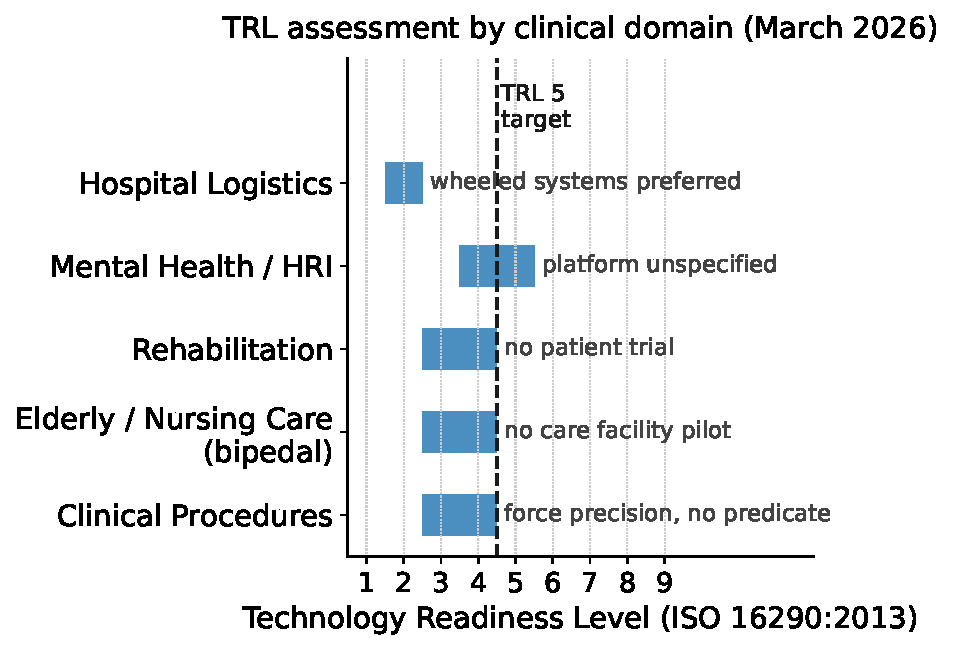
\includegraphics[width=\columnwidth]{figures/trl_readiness.pdf}
  \caption{Technology Readiness Level (TRL) assessment by clinical domain
  (March 2026). Current TRL range (filled bars) and TRL~5 target (dashed line)
  per ISO 16290:2013. No domain has reached TRL~7 (operational environment
  prototype); TRL~5 (relevant-environment validation) is the realistic five-year
  target for clinical procedures, elderly care (bipedal), and rehabilitation.}
  \label{fig:trl}
\end{figure}
\afterpage{\clearpage}

Figure~\ref{fig:radar} quantifies the specific capability gaps between the
current state-of-the-art and the required thresholds for two leading clinical
deployment domains.

\clearpage

\begin{figure}[H]
  \centering
  \Description{Radar chart with six axes: Force Precision, Gait Safety, Tactile
  Sensing, Tool Kinematics, AI Generalization, and Clinical Validation. Three
  overlapping polygon traces are shown: current state (blue, solid) with scores
  approximately 3--5 out of 10 on all axes; required threshold for clinical
  procedures (red, dashed) with scores 7--8; required threshold for elderly
  nursing care (green, dashed) with scores 5--8. The largest gap for both
  domains is in Clinical Validation (current score 1), followed by Gait Safety.}
  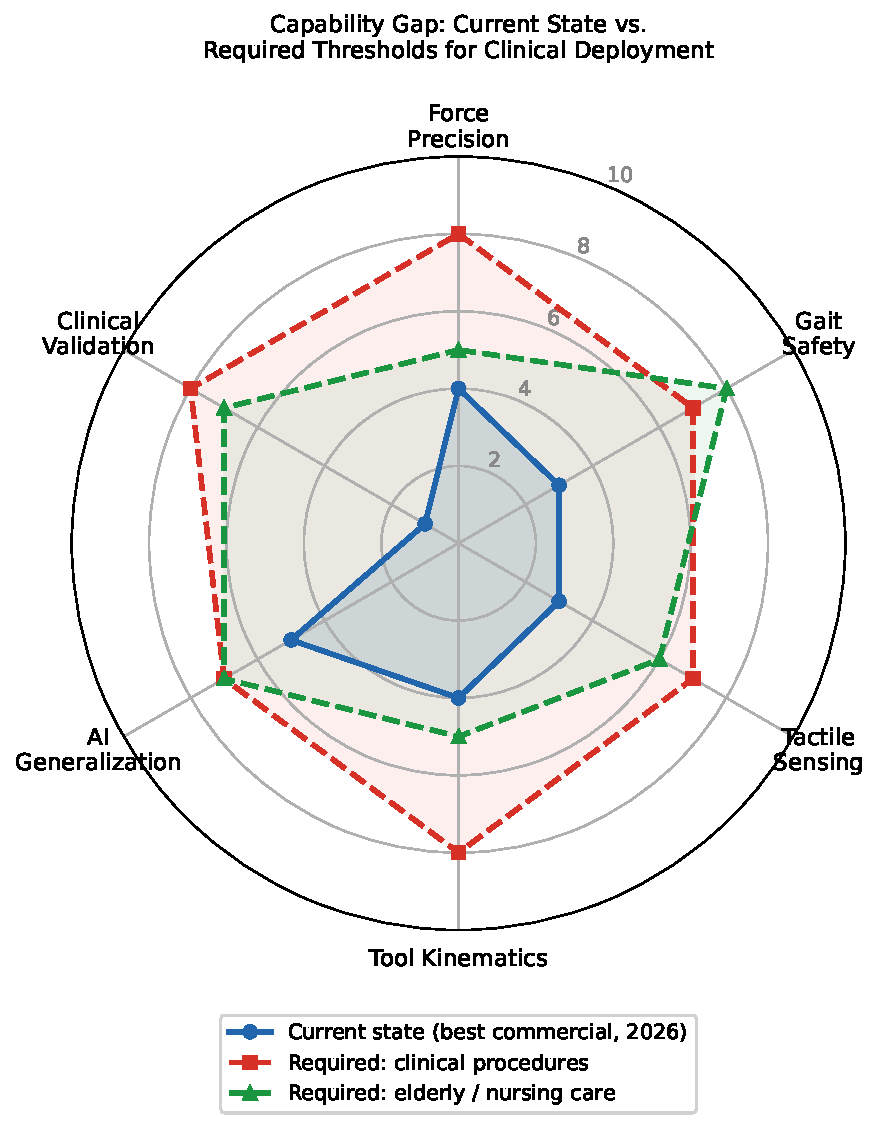
\includegraphics[width=0.6\columnwidth]{figures/capability_radar.pdf}
  \caption{Capability gap radar chart: current state-of-the-art (blue, 2026)
  versus required thresholds for clinical procedures (red dashed) and elderly
  nursing care (green dashed). Scores are on a 0--10 scale representing
  engineering and evidence maturity. Clinical Validation is the universal
  bottleneck (current score 1 of 10); Gait Safety is the dominant engineering
  gap for eldercare; Force Precision and Tool Kinematics are the key gaps for
  clinical procedure performance.}
  \label{fig:radar}
\end{figure}

\subsection{Near-Term Deployable Roles}
\label{sec:roles}

Three roles have the strongest case for TRL~5 achievement within five years.

\textbf{Role~1: Telemedicine and telepresence clinical assistant.} The teleoperated
mode is the key risk-mitigation design choice: by keeping a human operator in the
decision loop at all times, it avoids the regulatory classification and safety
validation burdens associated with autonomous patient contact. The technical
infrastructure exists: Atar et al.~\cite{atar2025humanoids} demonstrate
teleoperated clinical task execution across seven procedures, and Liang et
al.~\cite{liang2025lapsurgie} extend this to laparoscopic surgery. The primary
application is specialist access extension---enabling a remote specialist to
conduct a physical examination or assist in a procedure in a rural or low-resource
setting. Realizing this role at TRL~5 requires a defined physical examination
protocol, remote operator training standards, and IRB oversight.

\textbf{Role~2: Rehabilitation movement demonstrator.} This role requires no
direct patient contact: the humanoid demonstrates movements that the patient
observes or follows. The bipedal gait safety gap identified in
Section~\ref{sec:safety}---the most universally blocking technical
barrier---becomes irrelevant to this specific role, because the safety concern is
dynamic contact force during locomotion near patients, not movement observation at
distance. The neuroscientific rationale is grounded in P5's mirror neuron
evidence~\cite{nguyen2024eeg}; the clinical acceptability is established by P6's
case series~\cite{sobrepera2022feasibility}. Advancing requires a registered
feasibility trial adapting a NAO or Pepper protocol to a full-size bipedal
humanoid demonstrator in stroke rehabilitation.

\textbf{Role~3: Structured eldercare companion and physical assistant.} RHP
Friends~\cite{benallegue2025rhp} is the only platform designed specifically for
this role. The hybrid autonomous/teleoperated architecture---in which routine
tasks run autonomously and non-routine tasks are handed to a remote
operator---is the correct design for this deployment scenario. The SPRING
project~\cite{alamedapineda2024spring} provides the deployment methodology and
user-acceptance evaluation framework. Realizing this role at TRL~5 requires an
actual care facility pilot.

\subsection{Research Priorities}
\label{sec:research}

Four priorities, ordered by their blocking impact on the entire field:

\textbf{Priority~1: Clinical safety validation for bipedal gait in patient-contact
environments.} The four gait-induced contact risk scenarios documented in
Section~\ref{sec:safety} are not bounded by any existing standard. No IRB will
approve human-subject studies involving physical patient contact by a full-size
bipedal humanoid without instrumented biomechanical data on these force profiles
and an accepted safety standard or architectural safeguard. This is the single
most leverage-intensive investment the field can make: resolving it unblocks
physical patient-contact studies in all three leading domains simultaneously.

\textbf{Priority~2: Human-subject feasibility studies in leading applications.}
The cadaveric endoscopy study of Cho et al.~\cite{cho2026humanoid} is the current
clinical frontier. The specific next step is an IRB-approved, registered
feasibility study in a narrow indication with an explicit safety monitor protocol.
UC San Diego (Yip Laboratory) and Johns Hopkins are the natural sites.

\textbf{Priority~3: Open clinical demonstration dataset for VLA training.} No
public dataset of humanoid robot demonstrations in clinical or
clinical-simulated environments exists. Creating an open clinical demonstration
dataset---even using simulators and clinical task protocols with mannequins---would
unlock foundation model fine-tuning for clinical applications and enable the
broader research community to advance clinical policy learning.

\textbf{Priority~4: Platform diversification for evidence generalizability.} The
concentration of clinical procedure evidence on the Unitree G1 (P1, P2, P3) is a
scientific limitation. Replication of clinical task evaluations on RHP Friends,
TALOS, or other platforms would establish whether current findings are
platform-specific or generalizable to the bipedal humanoid class.

\clearpage
\subsection{Regulatory Roadmap}
\label{sec:roadmap}

Figure~\ref{fig:regulatory} illustrates the parallel regulatory tracks and their
key decision points for both jurisdictions.

\begin{figure}[H]
  \centering
  \Description{Two-column flowchart comparing the US FDA and EU regulatory
  pathways for a clinical humanoid robot. Left column (FDA): novel device with
  no predicate leads to De Novo pathway (21 CFR 513(f)(2)), Pre-Submission
  meeting, De Novo request submission with bench and clinical data, FDA review
  approximately 12 months, then Class II market authorization with post-market
  surveillance. Right column (EU): EU MDR Class IIb/III assessment with Notified
  Body, EU AI Act high-risk AI system conformity assessment (effective August
  2026), clinical investigation under MDR Article 62, CE marking plus AI Act
  declaration of conformity, then EU market authorization with post-market
  clinical follow-up. A red banner at the bottom highlights the critical gap in
  both tracks: no accepted safety standard exists for bipedal gait in
  patient-proximate environments, as ISO 13482 excludes medical devices and
  ISO/TS 15066 is designed for fixed-base collaborative arms.}
  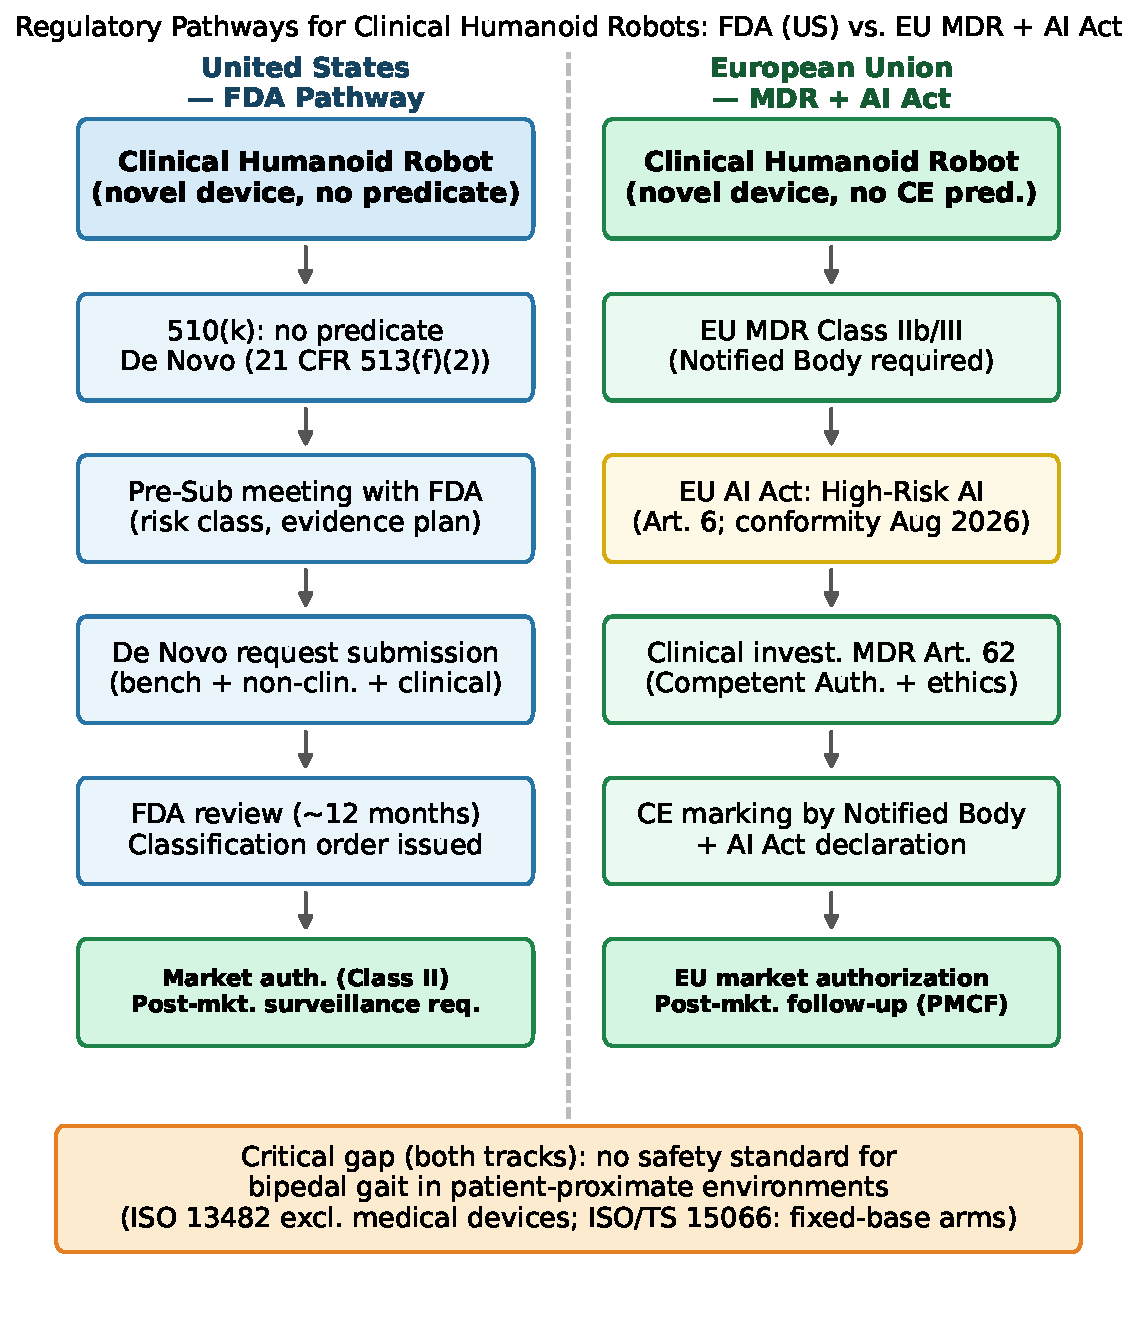
\includegraphics[width=\columnwidth]{figures/regulatory_pathways.pdf}
  \caption{Regulatory pathways for clinical humanoid robots: FDA De~Novo (US,
  left) and EU MDR plus EU AI Act (EU, right). Both tracks require the same
  foundational evidence---safety standards for bipedal gait in patient-proximate
  environments---that does not yet exist (bottom banner). FDA De~Novo is
  identified as the most plausible first-clearance pathway; EU MDR plus AI Act
  dual compliance represents the EU parallel track.}
  \label{fig:regulatory}
\end{figure}

The path to the first regulatory clearance requires three sequential steps.

\textbf{Step~1: Performance standards definition.} A joint effort among humanoid
manufacturers, academic medical centers (UCSD, JHU), and FDA's Center for Devices
and Radiological Health (CDRH) is required to define the Special Controls that
any De~Novo submission must meet: fall prevention performance requirements, patient
contact force limits for dynamic bipedal scenarios, teleoperation latency bounds,
and AI/ML software validation methodology consistent with FDA's Good Machine
Learning Practice principles and the December~2024 PCCP guidance.

\textbf{Step~2: IRB feasibility study generating clinical evidence.} A registered,
IRB-approved feasibility study in a specific narrow indication generates the
clinical evidence required for a De~Novo submission. This study must be designed
from the outset with regulatory submission in mind: pre-specified safety endpoints
and a defined safety monitor protocol.

\textbf{Step~3: De~Novo submission establishing a regulatory predicate.} The
De~Novo application proposes a new product code for bipedal humanoid clinical
assistants with Special Controls from Steps~1 and~2. First clearance establishes
a predicate device, enabling subsequent 510(k) applications.

For the EU, the parallel path requires: an ISO/TC~299 scope revision of
ISO~13482 to include clinical humanoids; EU MDR Class~IIa conformity assessment;
and EU AI Act compliance under high-risk AI obligations (effective August~2026 for
new AI systems; August~2027 for AI embedded in regulated medical products).
Regulatory precedents for navigating layered framework compliance exist in the
surgical robotics domain.

\subsection{Ethical Considerations}
\label{sec:ethics}

\textbf{Dignity of care.} Physical care interactions require that the patient
feels cared for, not processed. The SPRING project finding that participants cited
eye-level conversational positioning as important for dignified
interaction~\cite{alamedapineda2024spring} provides direct empirical evidence that
form factor affects perceived dignity of care. The uncanny valley phenomenon---the
negative affective response elicited by human-like but not fully human
entities~\cite{mori2012uncanny}---is particularly relevant for humanoid design in
care settings, where distress rather than curiosity is the cost of a poor
perceptual response. Care robotics designers must incorporate patient dignity
explicitly as a design criterion alongside technical performance metrics.

\textbf{Liability and informed consent.} No current healthcare liability
framework assigns accountability for harm caused by an autonomous or
semi-autonomous robotic action in a care setting. The ethical dimensions of robot
care for elderly individuals---including dignity, autonomy, and emotional
manipulation risks---require explicit frameworks before
deployment~\cite{sharkey2012granny}. Before any human-subject deployment, consent
processes for humanoid-assisted care must be defined. These require deliberate
engagement between legal, ethical, and clinical stakeholders before the first
human-subject study is launched.

\textbf{Data privacy.} A humanoid operating in a patient room integrates cameras,
microphones, depth sensors, physiological monitors, and, in future deployments,
integration with EHR systems, into a single mobile platform in one of the most
privacy-sensitive environments imaginable. No data governance framework specific
to clinical humanoid sensor data currently exists.

\textbf{Workforce framing.} The evidence does not support a displacement
narrative. No clinical role exists that a humanoid currently performs reliably
enough to replace a trained nurse or clinician. The evidence-supported framing is
task offloading: routine, physically demanding, or cognitively repetitive tasks
that do not require clinical judgment could be offloaded, freeing clinicians for
judgment-requiring activities. The administrator survey of Imtiaz and
Khan~\cite{imtiaz2024perceptions} shows that the perceived risk of reduced human
contact is a primary institutional barrier; communicating the task-offloading
framing accurately to institutional decision-makers is as important as resolving
the technical barriers.

%%======================================================================
\section{Conclusion}
\label{sec:conclusion}
%%======================================================================

As of March 2026, no bipedal humanoid robot holds FDA clearance or CE marking for
any clinical application. No registered Phase~I, II, or III clinical trial has
enrolled patients for a study involving a full-size bipedal humanoid platform. The
systematic search underlying this review identified 14 qualifying papers across
2022--2026---a literature sparse enough to read in its entirety, concentrated on a
single commercial platform (Unitree G1) and, for the clinically most advanced
domain, on a single research cluster (UCSD Yip Laboratory and Johns Hopkins). That
concentration is not evidence of a field in failure; it is evidence of a field in
its earliest phase of organized research. The infrastructure that would enable
distributed clinical investigation---accepted safety standards for bipedal
patient-contact environments, IRB-validated study protocols, and regulatory
pathways with established Special Controls---does not yet exist, and its absence
explains the concentration far better than any deficit of platform capability or
clinical motivation.

The contribution of this review is to document that gap with specificity
sufficient to act on it. Prior reviews of healthcare robotics, including the
closest comparative work in the literature~\cite{cunha2025humanoid}, either
predate the LLM/VLA inflection that is the enabling technical development of the
current period, or treat humanoid and non-humanoid platforms interchangeably,
obscuring the platform-specific barriers and advantages that define the clinical
deployment problem. The synthesis here is the first to integrate the full
2022--2026 humanoid-specific literature with a commercial and academic platform
capability assessment, a regulatory pathway analysis, and a per-domain TRL
readiness evaluation grounded in clinical deployment criteria.

The field is not uniform in its readiness. Three roles have a credible path to
first human-subject validation---TRL~5---within five years: a telemedicine and
telepresence clinical assistant operating in fully teleoperated mode, which
minimizes autonomous patient-contact risk and maps directly onto the established
regulatory logic of physician-controlled surgical robotics; a rehabilitation
movement demonstrator that exploits the mirror neuron mechanism established by
Nguyen et al.~\cite{nguyen2024eeg} and the clinical acceptability demonstrated by
Sobrepera et al.~\cite{sobrepera2022feasibility} without requiring any patient
contact, rendering the bipedal gait safety gap irrelevant to this role; and a
structured eldercare companion and physical assistant following the hybrid
autonomous/teleoperated architecture demonstrated by RHP
Friends~\cite{benallegue2025rhp} and the deployment methodology established by
the SPRING project~\cite{alamedapineda2024spring}. These are not speculative
roles. They are identified by triangulating the strongest evidence in the
literature, the most tractable technical barriers, and the lowest regulatory risk
profile available to each application.

Two gaps are more consequential than the others identified in
Section~\ref{sec:challenges}. The first is the absence of any accepted performance
standard for bipedal humanoid robots in patient-proximate environments---specifically
for the four categories of gait-induced contact events that ISO/TS~15066 was not
designed to address. This gap does not require a breakthrough to close; it
requires a biomechanical characterization study and the standards development
process. But no IRB will approve physical patient-contact studies without it, and
no regulatory agency can specify Special Controls without it. It is the single
most globally blocking gap in the field. The second is the absence of registered
human-subject feasibility studies. Cho et al.~\cite{cho2026humanoid} advance the
state of the art by completing a cadaveric surgical study under a defined IRB
protocol---the step immediately preceding first-in-human research. UC San Diego
and Johns Hopkins, which together hold all three papers in the clinical procedures
domain, are the natural sites for this next step. There is no institutional
reason, beyond the gait safety gap, why this study cannot begin within the current
funding cycle.

The question confronting the field is not whether humanoid robots can play a
useful role in healthcare. The evidence in this review establishes that they
can---not at the level of clinical deployment, but at the level of demonstrated
laboratory capability in procedures and care tasks that have genuine clinical
value. The question is whether the research community, device manufacturers,
clinical institutions, and regulatory agencies will commit to the specific,
sequential, methodical process required to convert that laboratory evidence into
clinical evidence, and clinical evidence into regulatory precedent. That
process---safety characterization, IRB feasibility study, De~Novo submission, and
predicate device establishment---is well understood in medical device development.
Applying it to a genuinely novel platform class, with novel form-factor dynamics
and novel AI system integration, requires institutional investment and coordination
that has not yet materialized at scale. The evidence base is ready for the next
step. The infrastructure to take it is the work of the next five years.

%%======================================================================
%% Acknowledgments
%%======================================================================
\begin{acks}
The authors thank [to be completed]. No external funding was received for this work.
\end{acks}

%%======================================================================
%% References
%%======================================================================
\bibliographystyle{ACM-Reference-Format}
\bibliography{references}

\end{document}
